% Options for packages loaded elsewhere
\PassOptionsToPackage{unicode}{hyperref}
\PassOptionsToPackage{hyphens}{url}
\documentclass[
]{book}
\usepackage{xcolor}
\usepackage{amsmath,amssymb}
\setcounter{secnumdepth}{5}
\usepackage{iftex}
\ifPDFTeX
  \usepackage[T1]{fontenc}
  \usepackage[utf8]{inputenc}
  \usepackage{textcomp} % provide euro and other symbols
\else % if luatex or xetex
  \usepackage{unicode-math} % this also loads fontspec
  \defaultfontfeatures{Scale=MatchLowercase}
  \defaultfontfeatures[\rmfamily]{Ligatures=TeX,Scale=1}
\fi
\usepackage{lmodern}
\ifPDFTeX\else
  % xetex/luatex font selection
\fi
% Use upquote if available, for straight quotes in verbatim environments
\IfFileExists{upquote.sty}{\usepackage{upquote}}{}
\IfFileExists{microtype.sty}{% use microtype if available
  \usepackage[]{microtype}
  \UseMicrotypeSet[protrusion]{basicmath} % disable protrusion for tt fonts
}{}
\makeatletter
\@ifundefined{KOMAClassName}{% if non-KOMA class
  \IfFileExists{parskip.sty}{%
    \usepackage{parskip}
  }{% else
    \setlength{\parindent}{0pt}
    \setlength{\parskip}{6pt plus 2pt minus 1pt}}
}{% if KOMA class
  \KOMAoptions{parskip=half}}
\makeatother
\usepackage{color}
\usepackage{fancyvrb}
\newcommand{\VerbBar}{|}
\newcommand{\VERB}{\Verb[commandchars=\\\{\}]}
\DefineVerbatimEnvironment{Highlighting}{Verbatim}{commandchars=\\\{\}}
% Add ',fontsize=\small' for more characters per line
\usepackage{framed}
\definecolor{shadecolor}{RGB}{248,248,248}
\newenvironment{Shaded}{\begin{snugshade}}{\end{snugshade}}
\newcommand{\AlertTok}[1]{\textcolor[rgb]{0.94,0.16,0.16}{#1}}
\newcommand{\AnnotationTok}[1]{\textcolor[rgb]{0.56,0.35,0.01}{\textbf{\textit{#1}}}}
\newcommand{\AttributeTok}[1]{\textcolor[rgb]{0.13,0.29,0.53}{#1}}
\newcommand{\BaseNTok}[1]{\textcolor[rgb]{0.00,0.00,0.81}{#1}}
\newcommand{\BuiltInTok}[1]{#1}
\newcommand{\CharTok}[1]{\textcolor[rgb]{0.31,0.60,0.02}{#1}}
\newcommand{\CommentTok}[1]{\textcolor[rgb]{0.56,0.35,0.01}{\textit{#1}}}
\newcommand{\CommentVarTok}[1]{\textcolor[rgb]{0.56,0.35,0.01}{\textbf{\textit{#1}}}}
\newcommand{\ConstantTok}[1]{\textcolor[rgb]{0.56,0.35,0.01}{#1}}
\newcommand{\ControlFlowTok}[1]{\textcolor[rgb]{0.13,0.29,0.53}{\textbf{#1}}}
\newcommand{\DataTypeTok}[1]{\textcolor[rgb]{0.13,0.29,0.53}{#1}}
\newcommand{\DecValTok}[1]{\textcolor[rgb]{0.00,0.00,0.81}{#1}}
\newcommand{\DocumentationTok}[1]{\textcolor[rgb]{0.56,0.35,0.01}{\textbf{\textit{#1}}}}
\newcommand{\ErrorTok}[1]{\textcolor[rgb]{0.64,0.00,0.00}{\textbf{#1}}}
\newcommand{\ExtensionTok}[1]{#1}
\newcommand{\FloatTok}[1]{\textcolor[rgb]{0.00,0.00,0.81}{#1}}
\newcommand{\FunctionTok}[1]{\textcolor[rgb]{0.13,0.29,0.53}{\textbf{#1}}}
\newcommand{\ImportTok}[1]{#1}
\newcommand{\InformationTok}[1]{\textcolor[rgb]{0.56,0.35,0.01}{\textbf{\textit{#1}}}}
\newcommand{\KeywordTok}[1]{\textcolor[rgb]{0.13,0.29,0.53}{\textbf{#1}}}
\newcommand{\NormalTok}[1]{#1}
\newcommand{\OperatorTok}[1]{\textcolor[rgb]{0.81,0.36,0.00}{\textbf{#1}}}
\newcommand{\OtherTok}[1]{\textcolor[rgb]{0.56,0.35,0.01}{#1}}
\newcommand{\PreprocessorTok}[1]{\textcolor[rgb]{0.56,0.35,0.01}{\textit{#1}}}
\newcommand{\RegionMarkerTok}[1]{#1}
\newcommand{\SpecialCharTok}[1]{\textcolor[rgb]{0.81,0.36,0.00}{\textbf{#1}}}
\newcommand{\SpecialStringTok}[1]{\textcolor[rgb]{0.31,0.60,0.02}{#1}}
\newcommand{\StringTok}[1]{\textcolor[rgb]{0.31,0.60,0.02}{#1}}
\newcommand{\VariableTok}[1]{\textcolor[rgb]{0.00,0.00,0.00}{#1}}
\newcommand{\VerbatimStringTok}[1]{\textcolor[rgb]{0.31,0.60,0.02}{#1}}
\newcommand{\WarningTok}[1]{\textcolor[rgb]{0.56,0.35,0.01}{\textbf{\textit{#1}}}}
\usepackage{longtable,booktabs,array}
\usepackage{calc} % for calculating minipage widths
% Correct order of tables after \paragraph or \subparagraph
\usepackage{etoolbox}
\makeatletter
\patchcmd\longtable{\par}{\if@noskipsec\mbox{}\fi\par}{}{}
\makeatother
% Allow footnotes in longtable head/foot
\IfFileExists{footnotehyper.sty}{\usepackage{footnotehyper}}{\usepackage{footnote}}
\makesavenoteenv{longtable}
\usepackage{graphicx}
\makeatletter
\newsavebox\pandoc@box
\newcommand*\pandocbounded[1]{% scales image to fit in text height/width
  \sbox\pandoc@box{#1}%
  \Gscale@div\@tempa{\textheight}{\dimexpr\ht\pandoc@box+\dp\pandoc@box\relax}%
  \Gscale@div\@tempb{\linewidth}{\wd\pandoc@box}%
  \ifdim\@tempb\p@<\@tempa\p@\let\@tempa\@tempb\fi% select the smaller of both
  \ifdim\@tempa\p@<\p@\scalebox{\@tempa}{\usebox\pandoc@box}%
  \else\usebox{\pandoc@box}%
  \fi%
}
% Set default figure placement to htbp
\def\fps@figure{htbp}
\makeatother
\setlength{\emergencystretch}{3em} % prevent overfull lines
\providecommand{\tightlist}{%
  \setlength{\itemsep}{0pt}\setlength{\parskip}{0pt}}
\usepackage[]{natbib}
\bibliographystyle{plainnat}
\usepackage{booktabs}
\usepackage{bookmark}
\IfFileExists{xurl.sty}{\usepackage{xurl}}{} % add URL line breaks if available
\urlstyle{same}
\hypersetup{
  pdftitle={Instrument Variables and Creating Variables},
  pdfauthor={Samuel Rowe},
  hidelinks,
  pdfcreator={LaTeX via pandoc}}

\title{Instrument Variables and Creating Variables}
\author{Samuel Rowe}
\date{2025-09-17}

\begin{document}
\maketitle

{
\setcounter{tocdepth}{1}
\tableofcontents
}
\begin{Shaded}
\begin{Highlighting}[]
\NormalTok{bookdown}\SpecialCharTok{::}\FunctionTok{serve\_book}\NormalTok{()}
\end{Highlighting}
\end{Shaded}

\chapter*{Overview}\label{overview}
\addcontentsline{toc}{chapter}{Overview}

\begin{enumerate}
\def\labelenumi{\arabic{enumi}.}
\tightlist
\item
  Instrumental Variables
\item
  Creating and Modifying Variables (Mitchell Chapter 6)
\end{enumerate}

Adapted from Mitchell (2020) and Wooldridge (2009)

\chapter{Instrumental Variables}\label{instrumental-variables}

Go to elms and download the mroz dta file.

\section{Estimating Returns to Education for Married Women}\label{estimating-returns-to-education-for-married-women}

We'll use the data from A. Mroz (1987), ``The Sensitivity of an Empirical Model of Married Women's Hours of Work to Economic and Statistical Assumptions,'' Econometrica 55, 765-799.

We'll use the data on married working women to estimate the return to education
using a simple OLS model.

Our likely biased OLS model results in the following

\begin{Shaded}
\begin{Highlighting}[]
\NormalTok{cd }\StringTok{"/Users/Sam/Desktop/Econ 645/Data/Wooldridge"}
\KeywordTok{use} \StringTok{"mroz.dta"}\NormalTok{, }\KeywordTok{clear}
\KeywordTok{reg}\NormalTok{ lwage educ}
\end{Highlighting}
\end{Shaded}

\begin{verbatim}
/Users/Sam/Desktop/Econ 645/Data/Wooldridge

      Source |       SS           df       MS      Number of obs   =       428
-------------+----------------------------------   F(1, 426)       =     56.93
       Model |  26.3264193         1  26.3264193   Prob > F        =    0.0000
    Residual |  197.001022       426  .462443713   R-squared       =    0.1179
-------------+----------------------------------   Adj R-squared   =    0.1158
       Total |  223.327441       427  .523015084   Root MSE        =    .68003

------------------------------------------------------------------------------
       lwage |      Coef.   Std. Err.      t    P>|t|     [95% Conf. Interval]
-------------+----------------------------------------------------------------
        educ |   .1086487   .0143998     7.55   0.000     .0803451    .1369523
       _cons |  -.1851968   .1852259    -1.00   0.318    -.5492673    .1788736
------------------------------------------------------------------------------
\end{verbatim}

Our estimate implies that the returns to education is exp(.109)-1*100 about 11.5\%. Notice that we are using stored values for \(\hat{\beta}_{edu}\) with \_b{[}edu{]}.

\begin{Shaded}
\begin{Highlighting}[]
\KeywordTok{display}\NormalTok{ (}\FunctionTok{exp}\NormalTok{(\_b[educ]){-}1)*100}
\end{Highlighting}
\end{Shaded}

\begin{verbatim}
11.477061
\end{verbatim}

We will use father's education as an instrument for the observation's level of education if the women is in the labor force. We will use the \emph{predict} command to get estimates of \(\hat{x}\)

\begin{Shaded}
\begin{Highlighting}[]
\KeywordTok{reg}\NormalTok{ educ fathedu }\KeywordTok{if}\NormalTok{ inlf==1}
\KeywordTok{predict}\NormalTok{ edu\_hat}
\end{Highlighting}
\end{Shaded}

\begin{verbatim}
      Source |       SS           df       MS      Number of obs   =       428
-------------+----------------------------------   F(1, 426)       =     88.84
       Model |  384.841983         1  384.841983   Prob > F        =    0.0000
    Residual |  1845.35428       426  4.33181756   R-squared       =    0.1726
-------------+----------------------------------   Adj R-squared   =    0.1706
       Total |  2230.19626       427  5.22294206   Root MSE        =    2.0813

------------------------------------------------------------------------------
        educ |      Coef.   Std. Err.      t    P>|t|     [95% Conf. Interval]
-------------+----------------------------------------------------------------
    fatheduc |   .2694416   .0285863     9.43   0.000     .2132538    .3256295
       _cons |   10.23705   .2759363    37.10   0.000     9.694685    10.77942
------------------------------------------------------------------------------

(option xb assumed; fitted values)
\end{verbatim}

For instrument relevance, let's obtain the F-Statistic after regressing education onto father's education.

\begin{Shaded}
\begin{Highlighting}[]
\KeywordTok{test}\NormalTok{ fathedu}
\end{Highlighting}
\end{Shaded}

\begin{verbatim}
 ( 1)  fatheduc = 0

       F(  1,   426) =   88.84
            Prob > F =    0.0000
\end{verbatim}

Our F-test shows that the instrument is greater than \(F-stat > 15\), so it seem like a relevant candidate for an instrument. This does not mean it is a good instrument, though.

Father's Education as an instrument

\begin{Shaded}
\begin{Highlighting}[]
\KeywordTok{reg}\NormalTok{ lwage edu\_hat}
\end{Highlighting}
\end{Shaded}

\begin{verbatim}
      Source |       SS           df       MS      Number of obs   =       428
-------------+----------------------------------   F(1, 426)       =      2.59
       Model |  1.34752449         1  1.34752449   Prob > F        =    0.1086
    Residual |  221.979916       426  .521079616   R-squared       =    0.0060
-------------+----------------------------------   Adj R-squared   =    0.0037
       Total |  223.327441       427  .523015084   Root MSE        =    .72186

------------------------------------------------------------------------------
       lwage |      Coef.   Std. Err.      t    P>|t|     [95% Conf. Interval]
-------------+----------------------------------------------------------------
     edu_hat |   .0591735   .0367969     1.61   0.109    -.0131525    .1314995
       _cons |   .4411034   .4671121     0.94   0.346    -.4770279    1.359235
------------------------------------------------------------------------------
\end{verbatim}

One additional year of education increases wages by \[ (e^{(0.059)}-1)*100\%=6.1\% \]

\begin{Shaded}
\begin{Highlighting}[]
\KeywordTok{display}\NormalTok{ (}\FunctionTok{exp}\NormalTok{(\_b[edu\_hat]){-}1)*100}
\end{Highlighting}
\end{Shaded}

\begin{verbatim}
6.095928
\end{verbatim}

Question?
The F-test passed the instrument relevance \(F-stat > 15\), but what
about instrument exogeneity?

\section{Exercise: Estimating Returns to Education for Men}\label{exercise-estimating-returns-to-education-for-men}

Let's estimate the returns to education for men. We'll use data from M. Blackburn and D. Neumark (1992), ``Unobserved Ability, Efficiency Wages, and Interindustry Wage Differentials,'' Quarterly Journal of Economics 107, 1421-1436.

Use number of siblings as an instrument to predict an observation's level of education. We'll keep it simple and have no other covariates.

\begin{enumerate}
\def\labelenumi{\arabic{enumi}.}
\tightlist
\item
  Estimate the potentially biased OLS
\item
  Estimate your first stage \(\hat{x}\)
\item
  Test your first stage
\item
  Run your second regression using \(\hat{x}\) from your first regression
\end{enumerate}

\begin{enumerate}
\def\labelenumi{\arabic{enumi})}
\tightlist
\item
  Estimate the potential biased OLS
\end{enumerate}

\begin{Shaded}
\begin{Highlighting}[]
\NormalTok{cd }\StringTok{"/Users/Sam/Desktop/Econ 645/Data/Wooldridge"}
\KeywordTok{use} \StringTok{"wage2.dta"}\NormalTok{, }\KeywordTok{clear}
\KeywordTok{reg}\NormalTok{ lwage educ}
\end{Highlighting}
\end{Shaded}

\begin{verbatim}
/Users/Sam/Desktop/Econ 645/Data/Wooldridge

      Source |       SS           df       MS      Number of obs   =       935
-------------+----------------------------------   F(1, 933)       =    100.70
       Model |  16.1377042         1  16.1377042   Prob > F        =    0.0000
    Residual |  149.518579       933  .160255712   R-squared       =    0.0974
-------------+----------------------------------   Adj R-squared   =    0.0964
       Total |  165.656283       934  .177362188   Root MSE        =    .40032

------------------------------------------------------------------------------
       lwage |      Coef.   Std. Err.      t    P>|t|     [95% Conf. Interval]
-------------+----------------------------------------------------------------
        educ |   .0598392   .0059631    10.03   0.000     .0481366    .0715418
       _cons |   5.973063   .0813737    73.40   0.000     5.813366    6.132759
------------------------------------------------------------------------------
\end{verbatim}

We have a estimated return of education of \[ (e^{.0598392}-1)*100\% = 6.2\% \]

\begin{Shaded}
\begin{Highlighting}[]
\KeywordTok{display}\NormalTok{ (}\FunctionTok{exp}\NormalTok{(\_b[educ]){-}1)*100}
\end{Highlighting}
\end{Shaded}

\begin{verbatim}
6.1665821
\end{verbatim}

\begin{enumerate}
\def\labelenumi{\arabic{enumi})}
\setcounter{enumi}{1}
\tightlist
\item
  Use Number of siblings as an instrument for the first stage and predict \(\hat{x}\)
\end{enumerate}

\begin{Shaded}
\begin{Highlighting}[]
\KeywordTok{reg}\NormalTok{ educ sibs}
\KeywordTok{predict}\NormalTok{ edu\_hat}
\end{Highlighting}
\end{Shaded}

\begin{verbatim}
      Source |       SS           df       MS      Number of obs   =       935
-------------+----------------------------------   F(1, 933)       =     56.67
       Model |  258.055048         1  258.055048   Prob > F        =    0.0000
    Residual |   4248.7642       933  4.55387374   R-squared       =    0.0573
-------------+----------------------------------   Adj R-squared   =    0.0562
       Total |  4506.81925       934  4.82528828   Root MSE        =     2.134

------------------------------------------------------------------------------
        educ |      Coef.   Std. Err.      t    P>|t|     [95% Conf. Interval]
-------------+----------------------------------------------------------------
        sibs |  -.2279164   .0302768    -7.53   0.000     -.287335   -.1684979
       _cons |   14.13879   .1131382   124.97   0.000     13.91676    14.36083
------------------------------------------------------------------------------

(option xb assumed; fitted values)
\end{verbatim}

\begin{enumerate}
\def\labelenumi{\arabic{enumi})}
\setcounter{enumi}{2}
\tightlist
\item
  Get F-statistic
\end{enumerate}

\begin{Shaded}
\begin{Highlighting}[]
\KeywordTok{test}\NormalTok{ sibs}
\end{Highlighting}
\end{Shaded}

\begin{verbatim}
 ( 1)  sibs = 0

       F(  1,   933) =   56.67
            Prob > F =    0.0000
\end{verbatim}

\begin{enumerate}
\def\labelenumi{\arabic{enumi})}
\setcounter{enumi}{3}
\tightlist
\item
  Number of siblings as an instrument
\end{enumerate}

\begin{Shaded}
\begin{Highlighting}[]
\KeywordTok{reg}\NormalTok{ lwage edu\_hat}
\end{Highlighting}
\end{Shaded}

\begin{verbatim}
      Source |       SS           df       MS      Number of obs   =       935
-------------+----------------------------------   F(1, 933)       =     22.31
       Model |  3.86818074         1  3.86818074   Prob > F        =    0.0000
    Residual |  161.788103       933  .173406326   R-squared       =    0.0234
-------------+----------------------------------   Adj R-squared   =    0.0223
       Total |  165.656283       934  .177362188   Root MSE        =    .41642

------------------------------------------------------------------------------
       lwage |      Coef.   Std. Err.      t    P>|t|     [95% Conf. Interval]
-------------+----------------------------------------------------------------
     edu_hat |   .1224326   .0259225     4.72   0.000     .0715595    .1733057
       _cons |   5.130026   .3494009    14.68   0.000     4.444323    5.815729
------------------------------------------------------------------------------
\end{verbatim}

One additional year of education increases wages by \[ (e^{0.1224}-1)*100\% =13.0\% \]

\begin{Shaded}
\begin{Highlighting}[]
\KeywordTok{display}\NormalTok{ (}\FunctionTok{exp}\NormalTok{(\_b[edu\_hat]){-}1)*100 }
\end{Highlighting}
\end{Shaded}

\begin{verbatim}
13.024298
\end{verbatim}

Another thing that is interesting here is the the OLS estimate is biased downward, which is not what we would expect.

Possible reasons:
1. Siblings could be correlated with ability - more siblings, less partental attention which could result in lower ability.
2. The OLS estimator is downward biased due to measurement error in educ, but this is less likely to satisfy the classic error-in-variables (CEM) assumption.

\section{Smoking on Birthweight}\label{smoking-on-birthweight}

It is important to see an example of a poor instrument. We'll use data from . Mullahy (1997), ``Instrumental-Variable Estimation of Count Data Models: Applications to Models of Cigarette Smoking Behavior,'' Review of Economics and Statistics 79, 596-593.

The biased OLS regression looks at the natural log of birth weight and cigarette packs smoked per day by the mother. We would expect that smoking is correlated with unobserved health and parental decisions, so it is like biased due to unobserved confounders.

\begin{Shaded}
\begin{Highlighting}[]
\NormalTok{cd }\StringTok{"/Users/Sam/Desktop/Econ 645/Data/Wooldridge"}
\KeywordTok{use} \StringTok{"bwght.dta"}\NormalTok{, }\KeywordTok{clear}
\KeywordTok{reg}\NormalTok{ lbwght packs}
\end{Highlighting}
\end{Shaded}

\begin{verbatim}
/Users/Sam/Desktop/Econ 645/Data/Wooldridge

      Source |       SS           df       MS      Number of obs   =     1,388
-------------+----------------------------------   F(1, 1386)      =     27.98
       Model |  .997781141         1  .997781141   Prob > F        =    0.0000
    Residual |  49.4225525     1,386  .035658407   R-squared       =    0.0198
-------------+----------------------------------   Adj R-squared   =    0.0191
       Total |  50.4203336     1,387  .036352079   Root MSE        =    .18883

------------------------------------------------------------------------------
      lbwght |      Coef.   Std. Err.      t    P>|t|     [95% Conf. Interval]
-------------+----------------------------------------------------------------
       packs |  -.0898131   .0169786    -5.29   0.000    -.1231197   -.0565065
       _cons |   4.769404   .0053694   888.26   0.000     4.758871    4.779937
------------------------------------------------------------------------------
\end{verbatim}

An additional package smoked per day decreases birthweight by \[ (e^{-.08981}-1)*100% \approx-8.6% 
\]

\begin{Shaded}
\begin{Highlighting}[]
\KeywordTok{display}\NormalTok{ (}\FunctionTok{exp}\NormalTok{({-}.08981){-}1)*100}
\end{Highlighting}
\end{Shaded}

\begin{verbatim}
-8.5895151
\end{verbatim}

We'll use cigarette prices as an instrument for cigarette packs smoked per day. We assume that cigarette prices and the error term u are uncorrelated (instrument exogeneity). Note that some states fund health care with cigarette tax revenue.
We will use cigarette price and quantity of packs smoked should be negatively
correlated.

\begin{Shaded}
\begin{Highlighting}[]
\KeywordTok{reg}\NormalTok{ packs cigprice}
\end{Highlighting}
\end{Shaded}

\begin{verbatim}
      Source |       SS           df       MS      Number of obs   =     1,388
-------------+----------------------------------   F(1, 1386)      =      0.13
       Model |  .011648626         1  .011648626   Prob > F        =    0.7179
    Residual |  123.684481     1,386  .089238442   R-squared       =    0.0001
-------------+----------------------------------   Adj R-squared   =   -0.0006
       Total |  123.696129     1,387  .089182501   Root MSE        =    .29873

------------------------------------------------------------------------------
       packs |      Coef.   Std. Err.      t    P>|t|     [95% Conf. Interval]
-------------+----------------------------------------------------------------
    cigprice |   .0002829    .000783     0.36   0.718    -.0012531    .0018188
       _cons |   .0674257   .1025384     0.66   0.511    -.1337215    .2685728
------------------------------------------------------------------------------
\end{verbatim}

The result shows that we fail to result the null hypothesis that \(\beta_{cigprice}\) is equal to 0. From theory, we know that something is wrong, since our instrument, price of cigarettes, is not associated with packs of cigarettes consumed.

We will still check instrument revelance:

\begin{Shaded}
\begin{Highlighting}[]
\KeywordTok{test}\NormalTok{ cigprice}
\end{Highlighting}
\end{Shaded}

\begin{verbatim}
 ( 1)  cigprice = 0

       F(  1,  1386) =    0.13
            Prob > F =    0.7179
\end{verbatim}

Our instrumennt fails the F-test - we have a \textbf{weak instrument}.

Cigarette price as an instrument for packs smoked is a poor instrument and our use of predicted packs smoked is in the wrong direction.

\begin{Shaded}
\begin{Highlighting}[]
\KeywordTok{predict}\NormalTok{ packs\_hat}
\KeywordTok{reg}\NormalTok{ lbwght packs\_hat}
\end{Highlighting}
\end{Shaded}

\begin{verbatim}
(option xb assumed; fitted values)

      Source |       SS           df       MS      Number of obs   =     1,388
-------------+----------------------------------   F(1, 1386)      =      2.87
       Model |  .104047659         1  .104047659   Prob > F        =    0.0907
    Residual |   50.316286     1,386  .036303237   R-squared       =    0.0021
-------------+----------------------------------   Adj R-squared   =    0.0013
       Total |  50.4203336     1,387  .036352079   Root MSE        =    .19053

------------------------------------------------------------------------------
      lbwght |      Coef.   Std. Err.      t    P>|t|     [95% Conf. Interval]
-------------+----------------------------------------------------------------
   packs_hat |   2.988676   1.765368     1.69   0.091    -.4744067    6.451758
       _cons |   4.448136   .1843027    24.13   0.000     4.086594    4.809679
------------------------------------------------------------------------------
\end{verbatim}

Our results show that something is terribly wrong. An additional package of cigarette is correlated with an massive increase in birth weight, which is not supported empirically. Our biased OLS was a better model than our poor instrument model.

We can and should always test Instrument Relevance. If we have a poor instrument, we should go back to the drawing board.

Another issue here is that price is a poor instrument, since price and quantity are simultaneously determined. We would need a second set of instruments on price to estimate our first-stage.

\section{Estimating Returns to Education for Married Women Part 2}\label{estimating-returns-to-education-for-married-women-part-2}

We'll use Mroz data again on working women. We'll use both parent's education as instruments to identify the effect of education on wages for working women. We overidentify the endogenous variable with two instruments: father's education and mother's education.

Potentially Biased OLS

\begin{Shaded}
\begin{Highlighting}[]
\NormalTok{cd }\StringTok{"/Users/Sam/Desktop/Econ 645/Data/Wooldridge"}
\KeywordTok{use} \StringTok{"mroz.dta"}\NormalTok{, }\KeywordTok{clear}
\KeywordTok{reg}\NormalTok{ lwage educ c.exper\#\#c.exper}
\end{Highlighting}
\end{Shaded}

\begin{verbatim}
/Users/Sam/Desktop/Econ 645/Data/Wooldridge

      Source |       SS           df       MS      Number of obs   =       428
-------------+----------------------------------   F(3, 424)       =     26.29
       Model |  35.0222967         3  11.6740989   Prob > F        =    0.0000
    Residual |  188.305144       424  .444115906   R-squared       =    0.1568
-------------+----------------------------------   Adj R-squared   =    0.1509
       Total |  223.327441       427  .523015084   Root MSE        =    .66642

---------------------------------------------------------------------------------
          lwage |      Coef.   Std. Err.      t    P>|t|     [95% Conf. Interval]
----------------+----------------------------------------------------------------
           educ |   .1074896   .0141465     7.60   0.000     .0796837    .1352956
          exper |   .0415665   .0131752     3.15   0.002     .0156697    .0674633
                |
c.exper#c.exper |  -.0008112   .0003932    -2.06   0.040    -.0015841   -.0000382
                |
          _cons |  -.5220406   .1986321    -2.63   0.009    -.9124667   -.1316144
---------------------------------------------------------------------------------
\end{verbatim}

Our result is \[ (e^{.1074896}-1)*100\% = 11.3\% \]

\begin{Shaded}
\begin{Highlighting}[]
\KeywordTok{display}\NormalTok{ (}\FunctionTok{exp}\NormalTok{(\_b[educ]){-}1)*100}
\end{Highlighting}
\end{Shaded}

\begin{verbatim}
11.347933
\end{verbatim}

We'll use two instruments for one endogenous variable, which will be parent's education as an instrument for women in the labor force.

\begin{Shaded}
\begin{Highlighting}[]
\KeywordTok{reg}\NormalTok{ educ c.exper\#\#c.exper fathedu mothedu }\KeywordTok{if}\NormalTok{ inlf==1}
\end{Highlighting}
\end{Shaded}

\begin{verbatim}
      Source |       SS           df       MS      Number of obs   =       428
-------------+----------------------------------   F(4, 423)       =     28.36
       Model |  471.620998         4   117.90525   Prob > F        =    0.0000
    Residual |  1758.57526       423  4.15738833   R-squared       =    0.2115
-------------+----------------------------------   Adj R-squared   =    0.2040
       Total |  2230.19626       427  5.22294206   Root MSE        =     2.039

---------------------------------------------------------------------------------
           educ |      Coef.   Std. Err.      t    P>|t|     [95% Conf. Interval]
----------------+----------------------------------------------------------------
          exper |   .0452254   .0402507     1.12   0.262    -.0338909    .1243417
                |
c.exper#c.exper |  -.0010091   .0012033    -0.84   0.402    -.0033744    .0013562
                |
       fatheduc |   .1895484   .0337565     5.62   0.000     .1231971    .2558997
       motheduc |    .157597   .0358941     4.39   0.000      .087044    .2281501
          _cons |    9.10264   .4265614    21.34   0.000     8.264196    9.941084
---------------------------------------------------------------------------------
\end{verbatim}

Get the F-Statistic.

\begin{Shaded}
\begin{Highlighting}[]
\KeywordTok{test}\NormalTok{ fathedu mothedu}
\end{Highlighting}
\end{Shaded}

\begin{verbatim}
 ( 1)  fatheduc = 0
 ( 2)  motheduc = 0

       F(  2,   423) =   55.40
            Prob > F =    0.0000
\end{verbatim}

The result shows that the instruments are potential candidates for good instruments, since \(F>15\).

Using Father's Education and Mother's Education as an instrument.

\begin{Shaded}
\begin{Highlighting}[]
\KeywordTok{predict}\NormalTok{ edu\_hat}
\KeywordTok{reg}\NormalTok{ lwage edu\_hat c.exper\#\#c.exper}
\end{Highlighting}
\end{Shaded}

\begin{verbatim}
(option xb assumed; fitted values)

      Source |       SS           df       MS      Number of obs   =       428
-------------+----------------------------------   F(3, 424)       =      7.40
       Model |   11.117828         3  3.70594265   Prob > F        =    0.0001
    Residual |  212.209613       424   .50049437   R-squared       =    0.0498
-------------+----------------------------------   Adj R-squared   =    0.0431
       Total |  223.327441       427  .523015084   Root MSE        =    .70746

---------------------------------------------------------------------------------
          lwage |      Coef.   Std. Err.      t    P>|t|     [95% Conf. Interval]
----------------+----------------------------------------------------------------
        edu_hat |   .0613966   .0329624     1.86   0.063    -.0033933    .1261866
          exper |   .0441704   .0140844     3.14   0.002     .0164865    .0718543
                |
c.exper#c.exper |   -.000899   .0004212    -2.13   0.033    -.0017268   -.0000711
                |
          _cons |   .0481003   .4197565     0.11   0.909    -.7769624     .873163
---------------------------------------------------------------------------------
\end{verbatim}

One additional year of education increases wages by \[ (e^{0.061}-1)*100\%=6.3\% \]

This can be more easily done with our \emph{ivregress 2sls} command:

\emph{ivregress 2sls} \emph{} (\emph{}=\emph{}) \(x_1, x_2...,x_k\)

\begin{Shaded}
\begin{Highlighting}[]
\NormalTok{ivregress 2sls lwage (educ=fathedu mothedu) c.exper\#\#c.exper}
\KeywordTok{display}\NormalTok{ (}\FunctionTok{exp}\NormalTok{(\_b[educ]){-}1)*100}
\end{Highlighting}
\end{Shaded}

\begin{verbatim}
Instrumental variables (2SLS) regression          Number of obs   =        428
                                                  Wald chi2(3)    =      24.65
                                                  Prob > chi2     =     0.0000
                                                  R-squared       =     0.1357
                                                  Root MSE        =     .67155

---------------------------------------------------------------------------------
          lwage |      Coef.   Std. Err.      z    P>|z|     [95% Conf. Interval]
----------------+----------------------------------------------------------------
           educ |   .0613966   .0312895     1.96   0.050     .0000704    .1227228
          exper |   .0441704   .0133696     3.30   0.001     .0179665    .0703742
                |
c.exper#c.exper |   -.000899   .0003998    -2.25   0.025    -.0016826   -.0001154
                |
          _cons |   .0481003    .398453     0.12   0.904    -.7328532    .8290538
---------------------------------------------------------------------------------
Instrumented:  educ
Instruments:   exper c.exper#c.exper fatheduc motheduc

6.3320574
\end{verbatim}

\chapter{Testing Assumptions}\label{testing-assumptions}

\section{Testing for Endogeneity - Returns to Education for Working Women}\label{testing-for-endogeneity---returns-to-education-for-working-women}

We'll keep using Mroz's data on working women.

Use father's and mother's education as an instrument to estimate education with the \emph{ivregress 2sls} command.

\begin{Shaded}
\begin{Highlighting}[]
\NormalTok{cd }\StringTok{"/Users/Sam/Desktop/Econ 645/Data/Wooldridge"}
\KeywordTok{use} \StringTok{"mroz.dta"}\NormalTok{, }\KeywordTok{clear}
\NormalTok{ivregress 2sls lwage (educ=fatheduc motheduc) c.exper\#\#c.exper}
\end{Highlighting}
\end{Shaded}

\begin{verbatim}
/Users/Sam/Desktop/Econ 645/Data/Wooldridge



Instrumental variables (2SLS) regression          Number of obs   =        428
                                                  Wald chi2(3)    =      24.65
                                                  Prob > chi2     =     0.0000
                                                  R-squared       =     0.1357
                                                  Root MSE        =     .67155

---------------------------------------------------------------------------------
          lwage |      Coef.   Std. Err.      z    P>|z|     [95% Conf. Interval]
----------------+----------------------------------------------------------------
           educ |   .0613966   .0312895     1.96   0.050     .0000704    .1227228
          exper |   .0441704   .0133696     3.30   0.001     .0179665    .0703742
                |
c.exper#c.exper |   -.000899   .0003998    -2.25   0.025    -.0016826   -.0001154
                |
          _cons |   .0481003    .398453     0.12   0.904    -.7328532    .8290538
---------------------------------------------------------------------------------
Instrumented:  educ
Instruments:   exper c.exper#c.exper fatheduc motheduc
\end{verbatim}

If want to see if our explanatory variable of interest is potentially
endogenous with the error term, then we can conduct an endogeneity test.
There are two ways to test for potential endogeneity in the OLS model

\begin{enumerate}
\def\labelenumi{\arabic{enumi}.}
\tightlist
\item
  Manually
\item
  \emph{estat} postestimation command
\end{enumerate}

\subsection{Manually Test}\label{manually-test}

To calculate the test manually, first we estimate the reduced form for \(\hat{x}_{edu}\) by regressing all exogenous variables onto \(x_{edu}\) by including all other \(x_{i}\) in the structural model and the additional IVs \(z_i\).

First, estimate the reduced form equation (first stage).

\begin{Shaded}
\begin{Highlighting}[]
\KeywordTok{reg}\NormalTok{ educ c.exper\#\#c.exper fathedu mothedu }\KeywordTok{if}\NormalTok{ inlf==1}
\end{Highlighting}
\end{Shaded}

\begin{verbatim}
      Source |       SS           df       MS      Number of obs   =       428
-------------+----------------------------------   F(4, 423)       =     28.36
       Model |  471.620998         4   117.90525   Prob > F        =    0.0000
    Residual |  1758.57526       423  4.15738833   R-squared       =    0.2115
-------------+----------------------------------   Adj R-squared   =    0.2040
       Total |  2230.19626       427  5.22294206   Root MSE        =     2.039

---------------------------------------------------------------------------------
           educ |      Coef.   Std. Err.      t    P>|t|     [95% Conf. Interval]
----------------+----------------------------------------------------------------
          exper |   .0452254   .0402507     1.12   0.262    -.0338909    .1243417
                |
c.exper#c.exper |  -.0010091   .0012033    -0.84   0.402    -.0033744    .0013562
                |
       fatheduc |   .1895484   .0337565     5.62   0.000     .1231971    .2558997
       motheduc |    .157597   .0358941     4.39   0.000      .087044    .2281501
          _cons |    9.10264   .4265614    21.34   0.000     8.264196    9.941084
---------------------------------------------------------------------------------
\end{verbatim}

Next, obtains residuals \(\hat{v}_2\).

\begin{Shaded}
\begin{Highlighting}[]
\KeywordTok{predict}\NormalTok{ v, residual}
\end{Highlighting}
\end{Shaded}

Then, add \(\hat{v}_2\) to the structural equation (our OLS model)

\begin{Shaded}
\begin{Highlighting}[]
\KeywordTok{reg}\NormalTok{ lwage educ c.exper\#\#c.exper v}
\end{Highlighting}
\end{Shaded}

\begin{verbatim}
      Source |       SS           df       MS      Number of obs   =       428
-------------+----------------------------------   F(4, 423)       =     20.50
       Model |  36.2573098         4  9.06432744   Prob > F        =    0.0000
    Residual |  187.070131       423  .442246173   R-squared       =    0.1624
-------------+----------------------------------   Adj R-squared   =    0.1544
       Total |  223.327441       427  .523015084   Root MSE        =    .66502

---------------------------------------------------------------------------------
          lwage |      Coef.   Std. Err.      t    P>|t|     [95% Conf. Interval]
----------------+----------------------------------------------------------------
           educ |   .0613966   .0309849     1.98   0.048      .000493    .1223003
          exper |   .0441704   .0132394     3.34   0.001     .0181471    .0701937
                |
c.exper#c.exper |   -.000899   .0003959    -2.27   0.024    -.0016772   -.0001208
                |
              v |   .0581666   .0348073     1.67   0.095    -.0102502    .1265834
          _cons |   .0481003   .3945753     0.12   0.903    -.7274721    .8236727
---------------------------------------------------------------------------------
\end{verbatim}

There is possible evidence of endogeneity since \(p < .1\) but \(p > .05\). You should report IV and OLS.

\begin{Shaded}
\begin{Highlighting}[]
\NormalTok{eststo m1: }\KeywordTok{quietly} \KeywordTok{reg}\NormalTok{ lwage educ c.exper\#\#c.exper}
\NormalTok{eststo m2: }\KeywordTok{quietly}\NormalTok{ ivregress 2sls lwage (educ=fatheduc motheduc) c.exper\#\#c.exper}
\NormalTok{esttab m1 m2, mtitle(OLS IV)}
\end{Highlighting}
\end{Shaded}

\begin{verbatim}
                      (1)             (2)   
                      OLS              IV   
--------------------------------------------
educ                0.107***       0.0614*  
                   (7.60)          (1.96)   

exper              0.0416**        0.0442***
                   (3.15)          (3.30)   

c.exper#c.~r    -0.000811*      -0.000899*  
                  (-2.06)         (-2.25)   

_cons              -0.522**        0.0481   
                  (-2.63)          (0.12)   
--------------------------------------------
N                     428             428   
--------------------------------------------
t statistics in parentheses
* p<0.05, ** p<0.01, *** p<0.001
\end{verbatim}

\subsection{Using estat endogenous}\label{using-estat-endogenous}

We can also use a postestimation command estat endogenous.

\begin{Shaded}
\begin{Highlighting}[]
\NormalTok{ivregress 2sls lwage (educ=fathedu mothedu) c.exper\#\#c.exper}
\KeywordTok{estat}\NormalTok{ endogenous}
\end{Highlighting}
\end{Shaded}

\begin{verbatim}
Instrumental variables (2SLS) regression          Number of obs   =        428
                                                  Wald chi2(3)    =      24.65
                                                  Prob > chi2     =     0.0000
                                                  R-squared       =     0.1357
                                                  Root MSE        =     .67155

---------------------------------------------------------------------------------
          lwage |      Coef.   Std. Err.      z    P>|z|     [95% Conf. Interval]
----------------+----------------------------------------------------------------
           educ |   .0613966   .0312895     1.96   0.050     .0000704    .1227228
          exper |   .0441704   .0133696     3.30   0.001     .0179665    .0703742
                |
c.exper#c.exper |   -.000899   .0003998    -2.25   0.025    -.0016826   -.0001154
                |
          _cons |   .0481003    .398453     0.12   0.904    -.7328532    .8290538
---------------------------------------------------------------------------------
Instrumented:  educ
Instruments:   exper c.exper#c.exper fatheduc motheduc


  Tests of endogeneity
  Ho: variables are exogenous

  Durbin (score) chi2(1)          =  2.80707  (p = 0.0938)
  Wu-Hausman F(1,423)             =  2.79259  (p = 0.0954)
\end{verbatim}

We have weak evidence that education is endogenous, since \(p<.1\) but \(p >.05\). However, we know from theory that ability is a confounder on wages and education. We should report both OLS and IV models.

\section{Testing Overidentifying Restrictions}\label{testing-overidentifying-restrictions}

We will testing overidentifying restrictions using the data from ``Returns to Education for Working Women''. When we have one IV for one endogenous explanatory variable, we have a just identified equation. When we have two instruments and one endogenous
explanatory variable we have overidentification.

When we have multiple IVs, we can test to see some of our instruments are correlated with the structural error term.

We can estimate two 2sls models (one for each IV) and then compare them. They should only differ by the sampling error. If our two beta coefficients on our fitted explanatory variable of interest are different then, we conclude that at least one instrument or maybe both is/are correlated with the structural error term.

When we add too many instrumental variables (or overidentification), we can increase the efficiency of the 2SLS estimator. However, we may run the risk of violating the instrument exogeneity assumption.

When we use motheredu and fatheredu as IVS for education, we have a single overidentification restriction. We have two IVs and 1 endogenous explanatory variable. We have two ways to calculate this test: manually and estat.

\subsection{Manually Test}\label{manually-test-1}

Use an 2SLS model with mother's education and father's education as two IVs.

\begin{Shaded}
\begin{Highlighting}[]
\NormalTok{cd }\StringTok{"/Users/Sam/Desktop/Econ 645/Data/Wooldridge"}
\KeywordTok{use} \StringTok{"mroz.dta"}\NormalTok{, }\KeywordTok{clear}
\NormalTok{ivregress 2sls lwage (educ=motheduc fatheduc) c.exper\#\#c.exper}
\end{Highlighting}
\end{Shaded}

\begin{verbatim}
/Users/Sam/Desktop/Econ 645/Data/Wooldridge



Instrumental variables (2SLS) regression          Number of obs   =        428
                                                  Wald chi2(3)    =      24.65
                                                  Prob > chi2     =     0.0000
                                                  R-squared       =     0.1357
                                                  Root MSE        =     .67155

---------------------------------------------------------------------------------
          lwage |      Coef.   Std. Err.      z    P>|z|     [95% Conf. Interval]
----------------+----------------------------------------------------------------
           educ |   .0613966   .0312895     1.96   0.050     .0000704    .1227228
          exper |   .0441704   .0133696     3.30   0.001     .0179665    .0703742
                |
c.exper#c.exper |   -.000899   .0003998    -2.25   0.025    -.0016826   -.0001154
                |
          _cons |   .0481003    .398453     0.12   0.904    -.7328532    .8290538
---------------------------------------------------------------------------------
Instrumented:  educ
Instruments:   exper c.exper#c.exper motheduc fatheduc
\end{verbatim}

Get our residuals \(r\) ane regress \(r\) onto all exogenous variables.

\begin{Shaded}
\begin{Highlighting}[]
\KeywordTok{predict} \FunctionTok{r}\NormalTok{, }\KeywordTok{resid}
\KeywordTok{reg} \FunctionTok{r}\NormalTok{ mothedu fathedu c.exper\#\#c.exper}
\end{Highlighting}
\end{Shaded}

\begin{verbatim}
(325 missing values generated)

      Source |       SS           df       MS      Number of obs   =       428
-------------+----------------------------------   F(4, 423)       =      0.09
       Model |  .170503122         4   .04262578   Prob > F        =    0.9845
    Residual |  192.849512       423  .455909012   R-squared       =    0.0009
-------------+----------------------------------   Adj R-squared   =   -0.0086
       Total |  193.020015       427  .452037506   Root MSE        =    .67521

---------------------------------------------------------------------------------
              r |      Coef.   Std. Err.      t    P>|t|     [95% Conf. Interval]
----------------+----------------------------------------------------------------
       motheduc |  -.0066065   .0118864    -0.56   0.579    -.0299704    .0167573
       fatheduc |   .0057823   .0111786     0.52   0.605    -.0161902    .0277547
          exper |  -.0000183   .0133291    -0.00   0.999    -.0262179    .0261813
                |
c.exper#c.exper |   7.34e-07   .0003985     0.00   0.999    -.0007825     .000784
                |
          _cons |   .0109641   .1412571     0.08   0.938    -.2666892    .2886173
---------------------------------------------------------------------------------
\end{verbatim}

Next, obtain \(R^2\) and \(N\)

\begin{Shaded}
\begin{Highlighting}[]
\KeywordTok{ereturn} \OtherTok{list}
\KeywordTok{local} \KeywordTok{N}\NormalTok{=}\OtherTok{\textasciigrave{}e(N)\textquotesingle{}}
\KeywordTok{display} \StringTok{"\textasciigrave{}N\textquotesingle{}"}
\KeywordTok{local}\NormalTok{ rsq=}\OtherTok{\textasciigrave{}e(r2)\textquotesingle{}}
\KeywordTok{display} \StringTok{"\textasciigrave{}rsq\textquotesingle{}"}
\KeywordTok{local}\NormalTok{ nR=}\OtherTok{\textasciigrave{}N\textquotesingle{}}\NormalTok{*}\OtherTok{\textasciigrave{}rsq\textquotesingle{}}
\KeywordTok{display} \StringTok{"\textasciigrave{}nR\textquotesingle{}"}
\end{Highlighting}
\end{Shaded}

\begin{verbatim}
scalars:
                  e(N) =  428
               e(df_m) =  4
               e(df_r) =  423
                  e(F) =  .0934962445404771
                 e(r2) =  .000883344256925
               e(rmse) =  .6752103466059415
                e(mss) =  .1705031219578643
                e(rss) =  192.8495121452517
               e(r2_a) =  -.0085645673813073
                 e(ll) =  -436.7021015142834
               e(ll_0) =  -436.891220726253
               e(rank) =  5

macros:
            e(cmdline) : "regress r mothedu fathedu c.exper##c.exper"
              e(title) : "Linear regression"
          e(marginsok) : "XB default"
                e(vce) : "ols"
             e(depvar) : "r"
                e(cmd) : "regress"
         e(properties) : "b V"
            e(predict) : "regres_p"
          e(estat_cmd) : "regress_estat"

matrices:
                  e(b) :  1 x 5
                  e(V) :  5 x 5

functions:
             e(sample)   


428


.000883344256925


.3780713419639
\end{verbatim}

Under the null hypothesis that all IVs are uncorrelated with \(u_1\)
\(NR^2 \thicksim \chi^2_{q}\), where \(q\) is the number of instruments from outside the model minus the total number of endogenous explanatory variables. If \(N R^2\) exceeds the 5\% critical value in \(\chi^2_q\), then we reject the null hypothesis and conclude that at least some of the IVs are not exogenous.

Here we have \(q=2-1=1\) df for the chi-squared test and we fail to reject the
null hypothesis since \(N R^2=0.37807\) and \(\chi^2_1\) at the 5\% critical value is 3.841.

\subsection{Estat overid}\label{estat-overid}

We can also use the postestimation command of \emph{estat overid}.

\begin{Shaded}
\begin{Highlighting}[]
\NormalTok{ivregress 2sls lwage (educ=motheduc fatheduc) c.exper\#\#c.exper}
\KeywordTok{estat}\NormalTok{ overid}
\end{Highlighting}
\end{Shaded}

\begin{verbatim}
Instrumental variables (2SLS) regression          Number of obs   =        428
                                                  Wald chi2(3)    =      24.65
                                                  Prob > chi2     =     0.0000
                                                  R-squared       =     0.1357
                                                  Root MSE        =     .67155

---------------------------------------------------------------------------------
          lwage |      Coef.   Std. Err.      z    P>|z|     [95% Conf. Interval]
----------------+----------------------------------------------------------------
           educ |   .0613966   .0312895     1.96   0.050     .0000704    .1227228
          exper |   .0441704   .0133696     3.30   0.001     .0179665    .0703742
                |
c.exper#c.exper |   -.000899   .0003998    -2.25   0.025    -.0016826   -.0001154
                |
          _cons |   .0481003    .398453     0.12   0.904    -.7328532    .8290538
---------------------------------------------------------------------------------
Instrumented:  educ
Instruments:   exper c.exper#c.exper motheduc fatheduc


  Tests of overidentifying restrictions:

  Sargan (score) chi2(1) =  .378071  (p = 0.5386)
  Basmann chi2(1)        =  .373985  (p = 0.5408)
\end{verbatim}

We get our \(N R^2\) with this postestimation command.

Let's add husband's education, so we have 2 overidentification restrictions.

\begin{Shaded}
\begin{Highlighting}[]
\NormalTok{ivregress 2sls lwage (educ=motheduc fatheduc huseduc) c.exper\#\#c.exper}
\KeywordTok{estat}\NormalTok{ overid}
\end{Highlighting}
\end{Shaded}

\begin{verbatim}
Instrumental variables (2SLS) regression          Number of obs   =        428
                                                  Wald chi2(3)    =      34.90
                                                  Prob > chi2     =     0.0000
                                                  R-squared       =     0.1495
                                                  Root MSE        =     .66616

---------------------------------------------------------------------------------
          lwage |      Coef.   Std. Err.      z    P>|z|     [95% Conf. Interval]
----------------+----------------------------------------------------------------
           educ |   .0803918    .021672     3.71   0.000     .0379155    .1228681
          exper |   .0430973   .0132027     3.26   0.001     .0172204    .0689742
                |
c.exper#c.exper |  -.0008628   .0003943    -2.19   0.029    -.0016357   -.0000899
                |
          _cons |  -.1868572   .2840591    -0.66   0.511    -.7436029    .3698885
---------------------------------------------------------------------------------
Instrumented:  educ
Instruments:   exper c.exper#c.exper motheduc fatheduc huseduc


  Tests of overidentifying restrictions:

  Sargan (score) chi2(2) =  1.11504  (p = 0.5726)
  Basmann chi2(2)        =  1.10228  (p = 0.5763)
\end{verbatim}

Notice that we still fail reject the null hypothesis, so we might consider adding it as an IV. Also, notice that the coefficient and standard error around education have changed as well.

It is a good idea to report both in a sensitivity analysis.

\begin{Shaded}
\begin{Highlighting}[]
\KeywordTok{est} \KeywordTok{clear}
\NormalTok{eststo m1: }\KeywordTok{quietly}\NormalTok{ ivregress 2sls lwage (educ=motheduc fatheduc) c.exper\#\#c.exper}
\NormalTok{eststo m2: }\KeywordTok{quietly}\NormalTok{ ivregress 2sls lwage (educ=motheduc fatheduc huseduc) c.exper\#\#c.exper}
\NormalTok{esttab m1 m2, mtitle(2IVs 3IVs)}
\end{Highlighting}
\end{Shaded}

\begin{verbatim}
                      (1)             (2)             (3)   
                      OLS            2IVs            3IVs   
------------------------------------------------------------
educ                0.107***       0.0614*         0.0804***
                   (7.60)          (1.96)          (3.71)   

exper              0.0416**        0.0442***       0.0431** 
                   (3.15)          (3.30)          (3.26)   

c.exper#c.~r    -0.000811*      -0.000899*      -0.000863*  
                  (-2.06)         (-2.25)         (-2.19)   

_cons              -0.522**        0.0481          -0.187   
                  (-2.63)          (0.12)         (-0.66)   
------------------------------------------------------------
N                     428             428             428   
------------------------------------------------------------
t statistics in parentheses
* p<0.05, ** p<0.01, *** p<0.001
\end{verbatim}

\chapter{Creating Variables}\label{creating-variables}

\textbf{Mitchell Chapter 6}

Overview
1. Generate and replace commands
2. Numeric expressions and functions
3. String expressions and functions
4. Recoding
5. Binary and Categorical variables
6. Date and Time functions
7. EGEN commands
8. Converting Strings to Numerics
9. Renaming and Reordering commands

The \emph{generate} and replace will be the workhorses of creating and modifying variables
We'll deal with generating binary variables. We'll look into missing data and how to handle it. \emph{Note: Please do not label your missing data, it just is a pain to deal with later}
The \emph{egen} command is also a very practical and useful (I wish other software
packages had this type of command). We'll deal with strings and converting between numerics and strings.

\section{Creating and changing variables}\label{creating-and-changing-variables}

One of the most basic tasks is to create, replace, and modify variables. Stata provides some nice and easy commands to work with variable generation and modification relative to other statistical software packages: \emph{generate} and \emph{replace}. These will be the workhorses for the creation and modification of variables.

As we go through Mitchell's Chapter 6, we'll see that these are not the only two commands we will utilize. For example, Stata has a very helpful command called \emph{egen}. It can be used to create new variables from old variables, especially when working with groups of observations. \emph{Egen} becomes even more helpful when it is combined with \emph{bysort}. We can sort our group and find the max, min, sum, etc. of a group of observations, which can come in handy when we are working with panel data. Futhermore, using indexes can make our generation commands more useful for creating lags or rebasing our data.

\subsection{Generate command}\label{generate-command}

The \emph{generate} or \emph{gen} command is one command that you may alredy have plenty of experience with, but there are some helpful tips when working with generate. What we'll do first is to create a new variable called potential experience and potential experience squared.

Let's look at ages for workers earning weekly wages.

\begin{Shaded}
\begin{Highlighting}[]
\NormalTok{cd }\StringTok{"/Users/Sam/Desktop/Data/CPS"}
\KeywordTok{use}\NormalTok{ smalljul25pub, }\KeywordTok{clear}
\KeywordTok{summarize}\NormalTok{ prtage }\KeywordTok{if}\NormalTok{ prerelg==1}
\KeywordTok{generate}\NormalTok{ pot\_exp=prtage{-}16}
\KeywordTok{summarize}\NormalTok{ pot\_exp }\KeywordTok{if}\NormalTok{ prerelg==1}
\end{Highlighting}
\end{Shaded}

\begin{verbatim}
/Users/Sam/Desktop/Data/CPS

    Variable |        Obs        Mean    Std. Dev.       Min        Max
-------------+---------------------------------------------------------
      prtage |      9,635    42.43778    14.74111         15         85

(28,617 missing values generated)

    Variable |        Obs        Mean    Std. Dev.       Min        Max
-------------+---------------------------------------------------------
     pot_exp |      9,635    26.43778    14.74111         -1         69
\end{verbatim}

Look for outliers and generate a histogram for outliers

\begin{Shaded}
\begin{Highlighting}[]
\KeywordTok{histogram}\NormalTok{ pot\_exp }\KeywordTok{if}\NormalTok{ prerelg==1}
\KeywordTok{graph} \KeywordTok{export} \StringTok{"jul\_25\_pot\_exp.png"}\NormalTok{, }\KeywordTok{replace}
\end{Highlighting}
\end{Shaded}

\begin{figure}
\centering
\pandocbounded{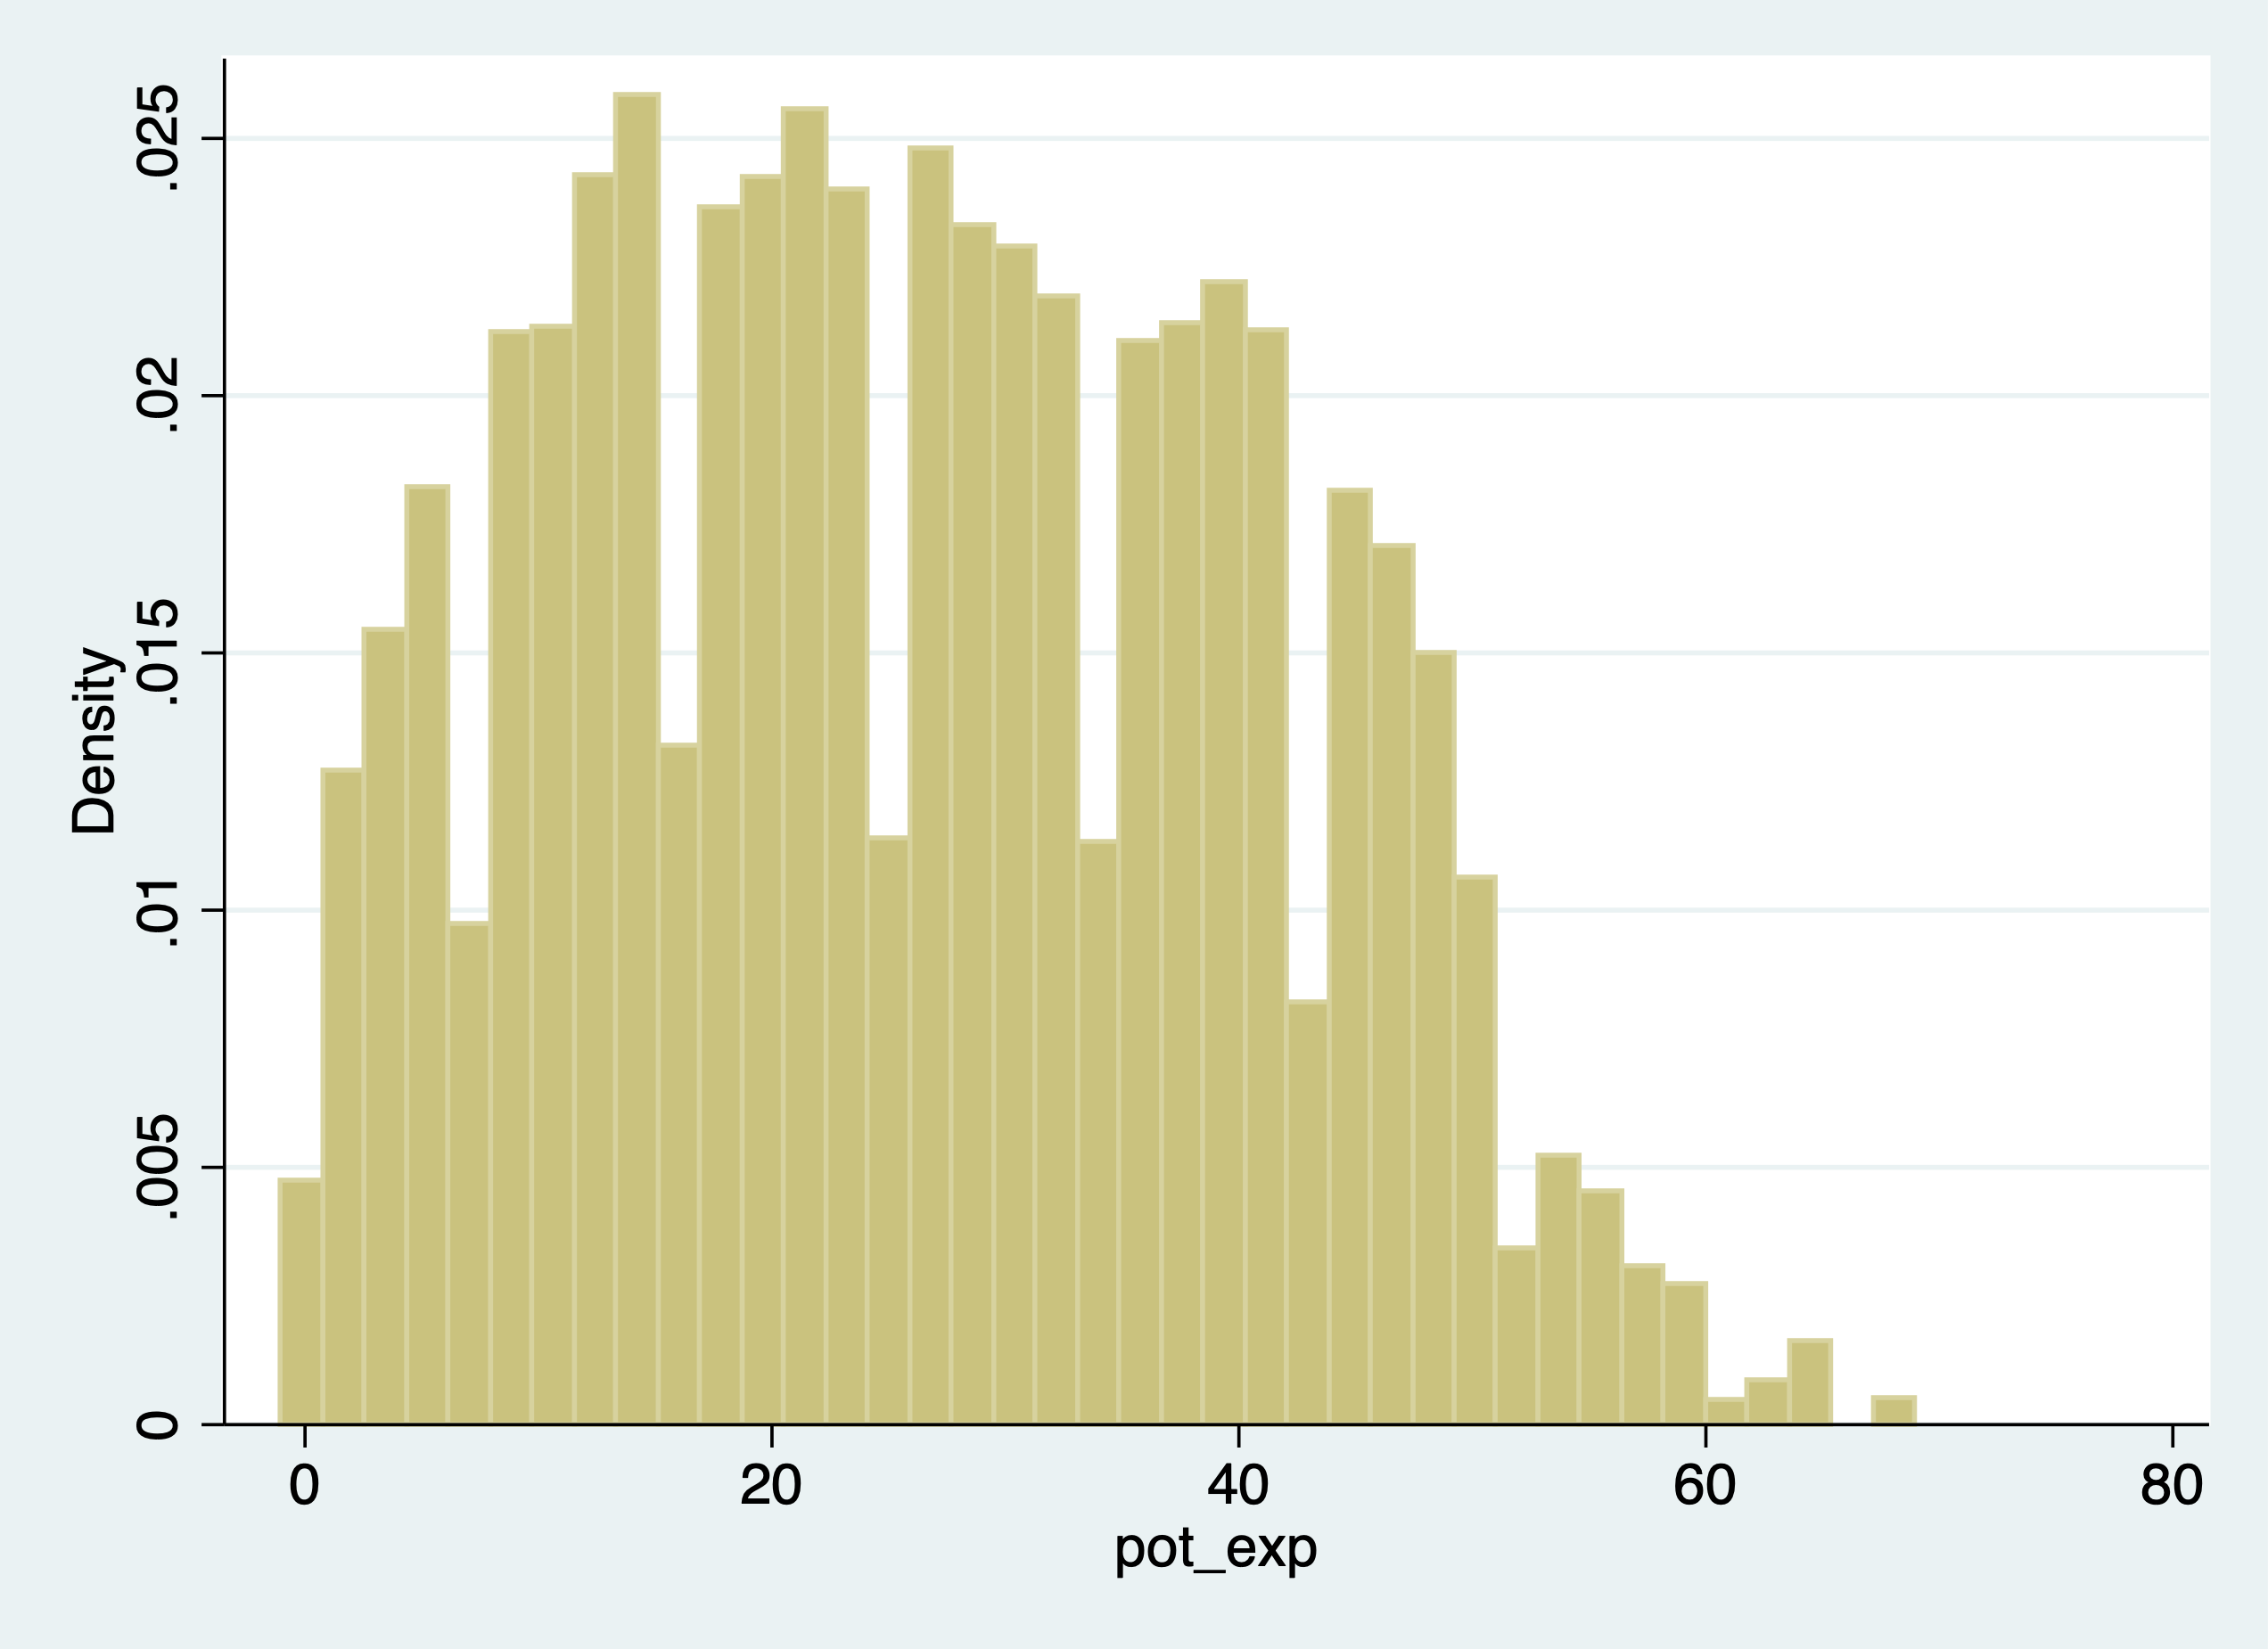
\includegraphics[keepaspectratio]{jul_25_pot_exp.png}}
\caption{Potential Experience}
\end{figure}

Now let's create a new variable for potential experience squared. We have two options:

\begin{Shaded}
\begin{Highlighting}[]
\KeywordTok{gen}\NormalTok{ pot\_exp2 = pot\_exp*pot\_exp}
\KeywordTok{sum}\NormalTok{ pot\_exp2}
\KeywordTok{drop}\NormalTok{ pot\_exp2}

\KeywordTok{gen}\NormalTok{ pot\_exp2 = pot\_exp\^{}2}
\KeywordTok{sum}\NormalTok{ pot\_exp2}
\end{Highlighting}
\end{Shaded}

\begin{verbatim}
(28,617 missing values generated)

    Variable |        Obs        Mean    Std. Dev.       Min        Max
-------------+---------------------------------------------------------
    pot_exp2 |     93,635    1269.006    1345.314          0       4761


(28,617 missing values generated)

    Variable |        Obs        Mean    Std. Dev.       Min        Max
-------------+---------------------------------------------------------
    pot_exp2 |     93,635    1269.006    1345.314          0       4761
\end{verbatim}

\textbf{Notice!} Our age variable, prtage, is missing whent the value is -1. The data dictionary provides us the information that -1 is a holder for missing data. Please note that when missing values are ``.'', we will see missings in an outlier check! Why? Because missing values are considered \textbf{very large values}. This is important because when creating binary or categorical variables through qualifiers, make sure you top code your qualifiers.

For example, if we are creating a binary on part-time vs full-time. We need to top code so we don't count missing hours as full-time workers,

\begin{Shaded}
\begin{Highlighting}[]
\KeywordTok{gen}\NormalTok{ fulltime }\KeywordTok{if}\NormalTok{ hours \textgreater{} 35 \& hours \textless{} 999999,}
\end{Highlighting}
\end{Shaded}

Alternatively, you can use the missing function.

\begin{Shaded}
\begin{Highlighting}[]
\KeywordTok{gen}\NormalTok{ fulltime }\KeywordTok{if}\NormalTok{ hours \textgreater{} 35 \& !}\FunctionTok{missing}\NormalTok{(hours)}
\end{Highlighting}
\end{Shaded}

Let's generate weekly earnings and plot the data. The CPS data dictionary tells us that pternwa is the weekly earnings, but it needs to be divided by 100 to get two decimal places.

\begin{Shaded}
\begin{Highlighting}[]
\KeywordTok{gen}\NormalTok{ earnings=pternwa/100}
\KeywordTok{histogram}\NormalTok{ earnings }\KeywordTok{if}\NormalTok{ prerelg==1, }\BaseNTok{title}\NormalTok{(Weekly Earnings)}
\KeywordTok{graph} \KeywordTok{export} \StringTok{"jul\_25\_weekly\_earnings.png"}\NormalTok{, }\KeywordTok{replace}
\end{Highlighting}
\end{Shaded}

\begin{figure}
\centering
\pandocbounded{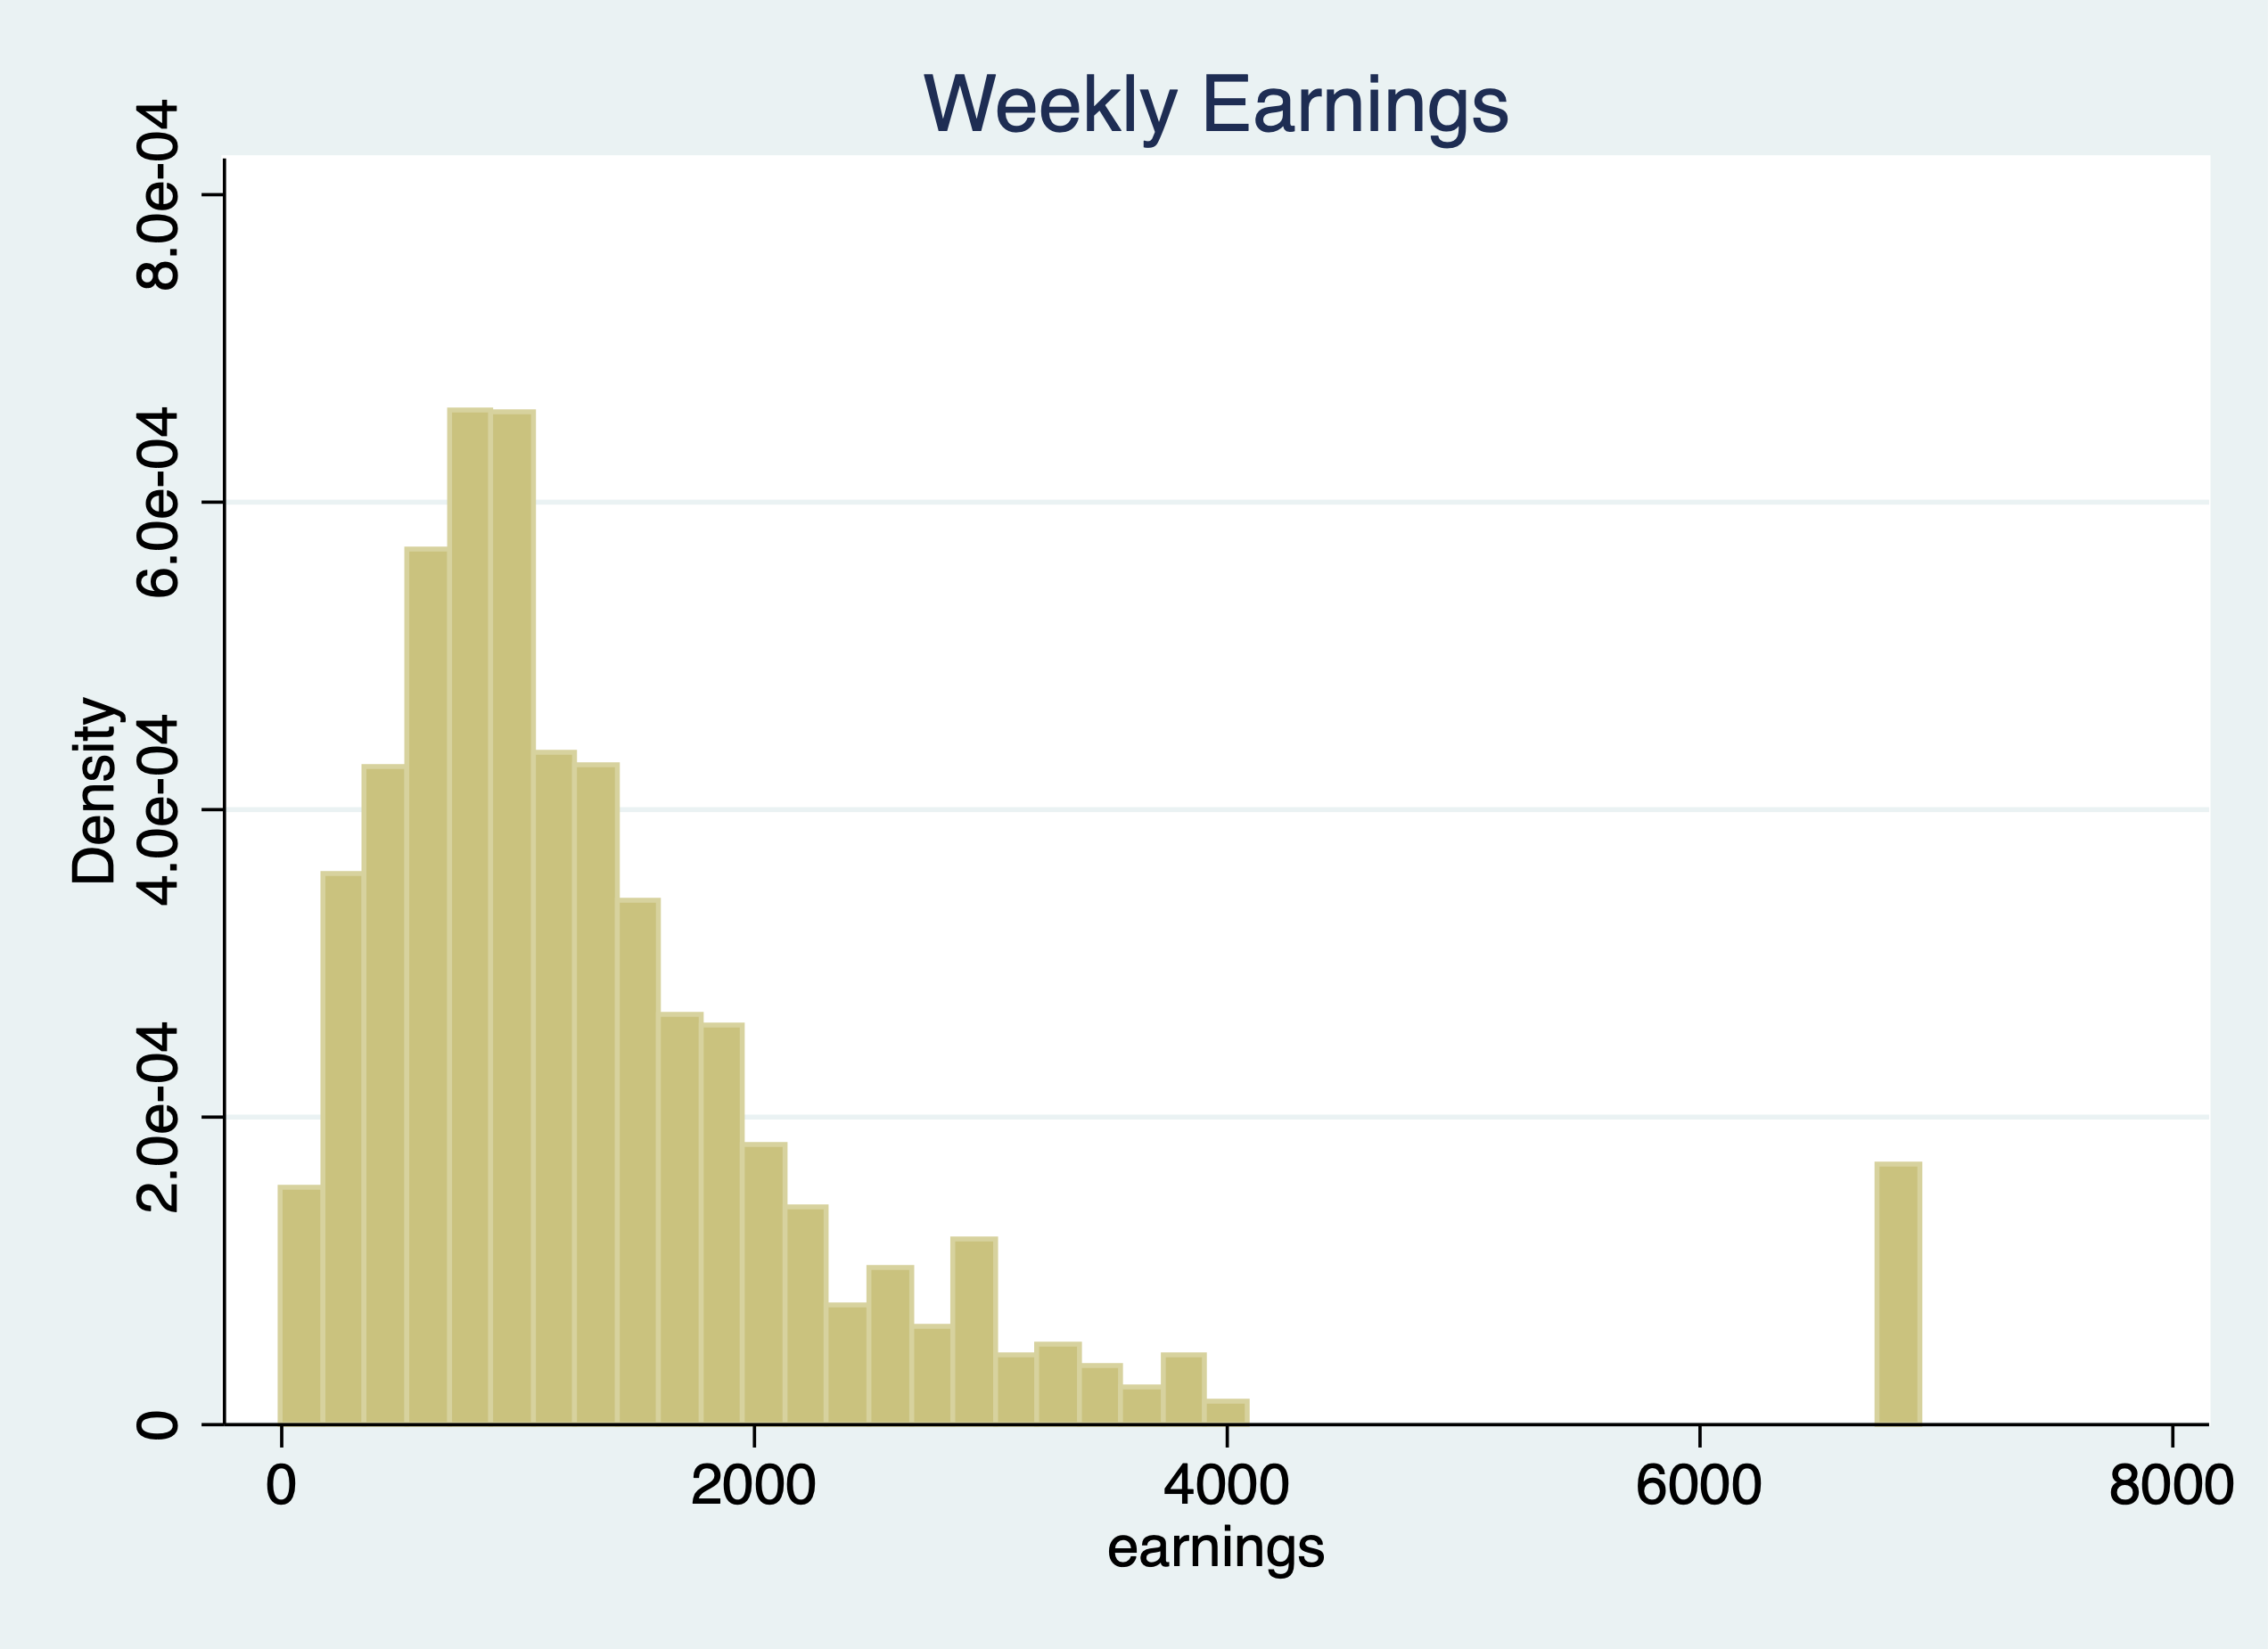
\includegraphics[keepaspectratio]{jul_25_weekly_earnings.png}}
\caption{Weekly Earnings}
\end{figure}

Another helpful trick is the before and after options. It might be helpful to have the newly created variable next to a similar variable, so let's drop our variable and generate it again with the after option

\begin{Shaded}
\begin{Highlighting}[]
\KeywordTok{drop}\NormalTok{ weekwage}
\KeywordTok{gen}\NormalTok{ hrlyearn = pternwa/pehract1, after(pternwa)}
\KeywordTok{drop}\NormalTok{ hrlyearn}
\KeywordTok{gen}\NormalTok{ hrlyearn = pternwa/pehract1, before(pternwa)}
\end{Highlighting}
\end{Shaded}

\subsection{Replace}\label{replace}

We use our \emph{replace} command to modify a variable that has already been created. Similar to generate, you probably already have experience with replace, but we'll go over some useful tips.

Qualifiers will be an essential part of your syntax when using the \emph{replace} command.

Let's generate a variable called marital status and look at married and nevermarried variables.

\begin{Shaded}
\begin{Highlighting}[]
\KeywordTok{quietly}\NormalTok{ cd }\StringTok{"/Users/Sam/Desktop/Econ 645/Data/Mitchell"}
\KeywordTok{quietly} \KeywordTok{use}\NormalTok{ wws, }\KeywordTok{clear}
\KeywordTok{tabulate}\NormalTok{ married nevermarried}
\end{Highlighting}
\end{Shaded}

\begin{verbatim}
           |   Woman never been
           |        married
   married |         0          1 |     Total
-----------+----------------------+----------
         0 |       570        234 |       804 
         1 |     1,440          2 |     1,442 
-----------+----------------------+----------
     Total |     2,010        236 |     2,246 
\end{verbatim}

We'll generate a new variable called maritalstatus.

\begin{Shaded}
\begin{Highlighting}[]
\KeywordTok{gen}\NormalTok{ maritalstatus = .}
\end{Highlighting}
\end{Shaded}

I recommend generating a new categorical variable as missing instead of zero, because this prevents missing variables from being categorized as 0 when applicable.

We generally use qualifers ``=, \textgreater, \textless, \textgreater=, \textless=, !'' when working with replace. Let's replace the marital status variable with married and nevermarried as qualifiers

\begin{Shaded}
\begin{Highlighting}[]
\KeywordTok{replace}\NormalTok{ maritalstatus = 1 }\KeywordTok{if}\NormalTok{ married==0 \& nevermarried==1}
\KeywordTok{replace}\NormalTok{ maritalstatus = 2 }\KeywordTok{if}\NormalTok{ married==1 \& nevermarried==0}
\KeywordTok{replace}\NormalTok{ maritalstatus = 3 }\KeywordTok{if}\NormalTok{ married==0 \& nevermarried==0}
\end{Highlighting}
\end{Shaded}

It's always a good idea to double check the varilabes against the variables they were created from to make sure your categories are what they are supposed to be.

\begin{Shaded}
\begin{Highlighting}[]
\KeywordTok{tabulate}\NormalTok{ maritalstatus}
\KeywordTok{table}\NormalTok{ maritalstatus married nevermarried}
\end{Highlighting}
\end{Shaded}

\begin{verbatim}
maritalstat |
         us |      Freq.     Percent        Cum.
------------+-----------------------------------
          1 |        234       10.43       10.43
          2 |      1,440       64.17       74.60
          3 |        570       25.40      100.00
------------+-----------------------------------
      Total |      2,244      100.00


----------------------------------------
          | Woman never been married and
          |           married           
maritalst | ----- 0 ----    ----- 1 ----
atus      |     0      1        0      1
----------+-----------------------------
        1 |                   234       
        2 |        1,440                
        3 |   570                       
----------------------------------------
\end{verbatim}

What will be helpful is to label our values, but we'll cover this next week.

We can also use the \emph{replace} command with a continuous variable in the qualifier

Let's create a new varible called over40hours which will be categorized as 1 if it is over 40 hours, and 0 if it is 40 or under.

\begin{Shaded}
\begin{Highlighting}[]
\KeywordTok{generate}\NormalTok{ over40hours = .}
\KeywordTok{replace}\NormalTok{ over40hours = 0 }\KeywordTok{if}\NormalTok{ hours \textless{}= 40}
\end{Highlighting}
\end{Shaded}

We need to make sure we don't include missing values so we need an additional qualifier besides hours \textgreater{} 40. We need to add !missing(hours).

\begin{Shaded}
\begin{Highlighting}[]
\KeywordTok{replace}\NormalTok{ over40hours = 1 }\KeywordTok{if}\NormalTok{ hours \textgreater{} 40 \& !}\FunctionTok{missing}\NormalTok{(hours)}
\end{Highlighting}
\end{Shaded}

Now let's see the results.

\begin{Shaded}
\begin{Highlighting}[]
\KeywordTok{tab}\NormalTok{ over40hours}
\KeywordTok{tab}\NormalTok{ over40hours, }\KeywordTok{sum}\NormalTok{(hours)}
\end{Highlighting}
\end{Shaded}

\begin{verbatim}
over40hours |      Freq.     Percent        Cum.
------------+-----------------------------------
          0 |      1,852       82.60       82.60
          1 |        390       17.40      100.00
------------+-----------------------------------
      Total |      2,242      100.00

            |    Summary of usual hours worked
over40hours |        Mean   Std. Dev.       Freq.
------------+------------------------------------
          0 |    34.50054   9.0449086       1,852
          1 |   50.123077   6.6961395         390
------------+------------------------------------
      Total |   37.218109   10.509135       2,242
\end{verbatim}

\section{Numeric expressions and functions}\label{numeric-expressions-and-functions}

Our standard numeric expressions
1. addition +,
2. subtraction -,
3. multiplication *,
4. division /,
5. exponentiation \^{}, and
6. parantheses () for changing order of operation.

We also have some very useful numeric functions built into Stata:

The \emph{int()} function removes any decimals.

The \emph{round()} function rounds a number to the desired decimal place.Please note that this is different from Excel!!!

The \emph{round(x,y)} rounds the numbers to the specified nearest value. Where x is your numeric and y is the nearest value you wish to round to.

For example:
1. if y = 1, round(-5.2,1)=-5 and round(4.5)=5
2. if y=.1, round(10.16,.1)=10.2 and round(34.1345,.1)=34.1
3. if y=10, round(313.34,10)=310 and round(4.52,10)=0

\textbf{Note:} if y is missing, then it will round to the nearest integer round(10.16)=10

The \emph{ln()} function is our natural log function which we use a lot for transforming variables for elasticity estimates.

The \emph{log10()} function is our logarithm base-10 function.

The \emph{sqrt()} function is our square root function

\begin{Shaded}
\begin{Highlighting}[]
    \KeywordTok{display} \KeywordTok{int}\NormalTok{(10.65)}
    \KeywordTok{display} \FunctionTok{round}\NormalTok{(10.65,1)}
    \KeywordTok{display} \FunctionTok{ln}\NormalTok{(10.65)}
    \KeywordTok{display} \FunctionTok{log10}\NormalTok{(10.65)}
    \KeywordTok{display} \FunctionTok{sqrt}\NormalTok{(10.65)}
\end{Highlighting}
\end{Shaded}

\begin{verbatim}
10

11

2.3655599

1.0273496

3.2634338
\end{verbatim}

Please note int(10.65) returns 10, while round(10.65,1) returns 11.

\subsection{Random Numbers and setting seeds}\label{random-numbers-and-setting-seeds}

There are several random number generating functions in Stata.

\emph{runiform()} is a random uniform distribution number generator has a distribution between 0 and 1.

\emph{rnormal(m,sd)} is a random normal distribution number generator without arguments it will assume mean = 0 and sd = 1.

\emph{rchi2(df)} is a random chi-squared distribution number generator where df is the degrees of freedom that need to be specified

Let's look at some examples.

Setting seeds is important if you want someone to replicate your results, since a set seed will generate the same random number each time it is run.

\begin{Shaded}
\begin{Highlighting}[]
\NormalTok{*Set our }\DecValTok{seed}
\KeywordTok{set} \DecValTok{seed}\NormalTok{ 12345}

\NormalTok{*Random uniform distribution }
\KeywordTok{gen}\NormalTok{ runiformtest = runiform()}
\KeywordTok{summarize}\NormalTok{ runiformtest}

\NormalTok{*Random }\FunctionTok{normal}\NormalTok{ distribution}
\KeywordTok{gen}\NormalTok{ rnormaltest = rnormal()}
\KeywordTok{gen}\NormalTok{ rnormaltest2 = rnormal(100,15)}
\KeywordTok{summarize}\NormalTok{ rnormaltest rnormaltest2}

\NormalTok{*Random chi{-}squared distribution}
\KeywordTok{gen}\NormalTok{ rchi2test = rchi2(5)}
\KeywordTok{summarize}\NormalTok{ rchi2test}
\end{Highlighting}
\end{Shaded}

\begin{verbatim}
    Variable |        Obs        Mean    Std. Dev.       Min        Max
-------------+---------------------------------------------------------
runiformtest |      2,246    .4924636    .2875376   .0007583   .9985869

    Variable |        Obs        Mean    Std. Dev.       Min        Max
-------------+---------------------------------------------------------
 rnormaltest |      2,246     .018436    .9857847  -3.389103   3.372525
rnormaltest2 |      2,246    99.70718    14.77732   47.81653   154.2297

    Variable |        Obs        Mean    Std. Dev.       Min        Max
-------------+---------------------------------------------------------
   rchi2test |      2,246    5.063639    3.322998   .1102785   29.24291
\end{verbatim}

\section{String Expressions and functions}\label{string-expressions-and-functions}

Working with string can be a pain, but there are some very helpful functions that will get your task completed.

\begin{Shaded}
\begin{Highlighting}[]
\KeywordTok{help} \FunctionTok{string}\NormalTok{ functions}
\end{Highlighting}
\end{Shaded}

Let's get some new data to work with strings and their functions.

We'll format the names with left-justification 17 characters long.

\begin{Shaded}
\begin{Highlighting}[]
\KeywordTok{quietly}\NormalTok{ cd }\StringTok{"/Users/Sam/Desktop/Econ 645/Data/Mitchell"}
\KeywordTok{use} \StringTok{"authors.dta"}\NormalTok{, }\KeywordTok{clear}    
\KeywordTok{format} \BaseNTok{name}\NormalTok{ \%{-}17s}
\OtherTok{list} \BaseNTok{name} 
\end{Highlighting}
\end{Shaded}

\begin{verbatim}
     | name                 |
     |----------------------|
  1. |  Ruth Canaale        |
  2. | Y. Don Uflossmore    |
  3. | thích nhất hạnh      |
  4. | J. Carreño Quiñones  |
  5. | Ô Knausgård          |
     |----------------------|
  6. | Don b Iteme          |
  7. | isaac O'yerbreath    |
  8. | Mike avity           |
  9. |      ÉMILE ZOLA      |
 10. | i William Crown      |
     |----------------------|
 11. | Ott W. Onthurt       |
 12. | Olive Tu'Drill       |
 13. | björk guðmundsdóttir |
     +----------------------+
\end{verbatim}

Notice white space(s) in front of some names and some names are not in the proper format (lowercase for initial letter instead of upper).

To fix these, we have a three string functions to work with.

The \emph{ustrtitle()} function is the Unicode function to convert strings to title cases, which means that the first letter is always upper and all others are lower case for each word.

The \emph{ustrlower()} is the Unicode function to convert strings to lower case.

The \emph{ustrupper()} is the Unicode function to convert strings to upper case.

Please note that there are string function that do something similar but in ASCII. Our names are not in ASCII currently, so please note that not all string characters come in ASCII, but may come in Unicode:
1. \emph{strproper()}
2. \emph{strlower()}
3. \emph{strupper()}

We'll generate some names and format our strings to 23 length and left-justified

\begin{Shaded}
\begin{Highlighting}[]
\KeywordTok{generate}\NormalTok{ name2 = ustrtitle(}\BaseNTok{name}\NormalTok{)}
\KeywordTok{generate}\NormalTok{ lowname = ustrlower(}\BaseNTok{name}\NormalTok{)}
\KeywordTok{generate}\NormalTok{ upname = ustrupper(}\BaseNTok{name}\NormalTok{)}
\KeywordTok{format}\NormalTok{ name2 lowname upname \%{-}23s}
\OtherTok{list}\NormalTok{ name2 lowname upname}
\end{Highlighting}
\end{Shaded}

\begin{verbatim}
     | name2                  lowname                upname               |
     |--------------------------------------------------------------------|
  1. |  Ruth Canaale           ruth canaale           RUTH CANAALE        |
  2. | Y. Don Uflossmore      y. don uflossmore      Y. DON UFLOSSMORE    |
  3. | Thích Nhất Hạnh        thích nhất hạnh        THÍCH NHẤT HẠNH      |
  4. | J. Carreño Quiñones    j. carreño quiñones    J. CARREÑO QUIÑONES  |
  5. | Ô Knausgård            ô knausgård            Ô KNAUSGÅRD          |
     |--------------------------------------------------------------------|
  6. | Don B Iteme            don b iteme            DON B ITEME          |
  7. | Isaac O'yerbreath      isaac o'yerbreath      ISAAC O'YERBREATH    |
  8. | Mike Avity             mike avity             MIKE AVITY           |
  9. |      Émile Zola             émile zola             ÉMILE ZOLA      |
 10. | I William Crown        i william crown        I WILLIAM CROWN      |
     |--------------------------------------------------------------------|
 11. | Ott W. Onthurt         ott w. onthurt         OTT W. ONTHURT       |
 12. | Olive Tu'drill         olive tu'drill         OLIVE TU'DRILL       |
 13. | Björk Guðmundsdóttir   björk guðmundsdóttir   BJÖRK GUÐMUNDSDÓTTIR |
     +--------------------------------------------------------------------+
\end{verbatim}

We still need to get rid of leading white spaces in front of the name. The \emph{ustrltrim()} will get reid of leading blanks.

\begin{Shaded}
\begin{Highlighting}[]
\KeywordTok{generate}\NormalTok{ name3 = ustrltrim(name2)}
\KeywordTok{format}\NormalTok{ name2 name3 \%{-}17s}
\OtherTok{list} \BaseNTok{name}\NormalTok{ name2 name3}
\end{Highlighting}
\end{Shaded}

\begin{verbatim}
     | name                   name2                  name3                |
     |--------------------------------------------------------------------|
  1. |  Ruth Canaale           Ruth Canaale          Ruth Canaale         |
  2. | Y. Don Uflossmore      Y. Don Uflossmore      Y. Don Uflossmore    |
  3. | thích nhất hạnh        Thích Nhất Hạnh        Thích Nhất Hạnh      |
  4. | J. Carreño Quiñones    J. Carreño Quiñones    J. Carreño Quiñones  |
  5. | Ô Knausgård            Ô Knausgård            Ô Knausgård          |
     |--------------------------------------------------------------------|
  6. | Don b Iteme            Don B Iteme            Don B Iteme          |
  7. | isaac O'yerbreath      Isaac O'yerbreath      Isaac O'yerbreath    |
  8. | Mike avity             Mike Avity             Mike Avity           |
  9. |      ÉMILE ZOLA             Émile Zola        Émile Zola           |
 10. | i William Crown        I William Crown        I William Crown      |
     |--------------------------------------------------------------------|
 11. | Ott W. Onthurt         Ott W. Onthurt         Ott W. Onthurt       |
 12. | Olive Tu'Drill         Olive Tu'drill         Olive Tu'drill       |
 13. | björk guðmundsdóttir   Björk Guðmundsdóttir   Björk Guðmundsdóttir |
     +--------------------------------------------------------------------+
\end{verbatim}

Let's work with the initials to identify the initial. In small datasets this is easy enough, but for large datasets we'll need to use some functions.

\subsection{substr functions}\label{substr-functions}

One of the more practical string functions is the substr functions:

The \emph{usubstr(s,n1,n2)} is our Unicode substring.

The \emph{substr(s,n1,n2)} is our ASCII substring

Where s is the string, n1 is the starting position, n2 is the length

\begin{Shaded}
\begin{Highlighting}[]
    \KeywordTok{display} \FunctionTok{substr}\NormalTok{(}\StringTok{"abcdef"}\NormalTok{,2,3)}
\end{Highlighting}
\end{Shaded}

\begin{verbatim}
bcd
\end{verbatim}

Let's find names that start with the initial with substr. We'll start at the 2nd position and move 1 character. Let's use ASCII and compare it to Unicode.

\begin{Shaded}
\begin{Highlighting}[]
\KeywordTok{gen}\NormalTok{ secondchar = }\FunctionTok{substr}\NormalTok{(name3,2,1)}
\KeywordTok{gen}\NormalTok{ firstinit = (secondchar == }\StringTok{" "}\NormalTok{ | secondchar == }\StringTok{"."}\NormalTok{) }\KeywordTok{if}\NormalTok{ !}\FunctionTok{missing}\NormalTok{(secondchar)}
\end{Highlighting}
\end{Shaded}

We might want to break up a string as well. This is helpful for names, addresses, etc.
We can use the strwordcount function.

The \emph{ustrwordcount(s)} counts the number of words using word-boundary rules of Unicode strings. Where s is the string input.

\begin{Shaded}
\begin{Highlighting}[]
\KeywordTok{generate}\NormalTok{ namecount = ustrwordcount(name3)}
\OtherTok{list}\NormalTok{ name3 namecount}
\end{Highlighting}
\end{Shaded}

\begin{verbatim}
     | name3                  nameco~t |
     |---------------------------------|
  1. | Ruth Canaale                  2 |
  2. | Y. Don Uflossmore             4 |
  3. | Thích Nhất Hạnh               3 |
  4. | J. Carreño Quiñones           4 |
  5. | Ô Knausgård                   2 |
     |---------------------------------|
  6. | Don B Iteme                   3 |
  7. | Isaac O'yerbreath             2 |
  8. | Mike Avity                    2 |
  9. | Émile Zola                    2 |
 10. | I William Crown               3 |
     |---------------------------------|
 11. | Ott W. Onthurt                4 |
 12. | Olive Tu'drill                2 |
 13. | Björk Guðmundsdóttir          2 |
     +---------------------------------+
\end{verbatim}

Notice that there are three authors have a word count of 4 instead of 3 when it should be three.

To extract the words after word count, we can use the \emph{ustrword()} command.
\emph{ustrword(s,n)} returns the word in the string depending upon n.~
\textbf{Note:} a positive n returns the nth word from the left, while a -n returns the nth word from the right.

\begin{Shaded}
\begin{Highlighting}[]
    \KeywordTok{generate}\NormalTok{ uname1=ustrword(name3,1)}
    \KeywordTok{generate}\NormalTok{ uname2=ustrword(name3,2)}
    \KeywordTok{generate}\NormalTok{ uname3=ustrword(name3,3)}
    \KeywordTok{generate}\NormalTok{ uname4=ustrword(name3,4)}
    \OtherTok{list}\NormalTok{ name3 uname1 uname2 uname3 uname4 namecount}
\end{Highlighting}
\end{Shaded}

\begin{verbatim}
(7 missing values generated)

(10 missing values generated)

     +----------------------------------------------------------------------------------+
     | name3                  uname1           uname2    uname3       uname4   nameco~t |
     |----------------------------------------------------------------------------------|
  1. | Ruth Canaale             Ruth          Canaale                                 2 |
  2. | Y. Don Uflossmore           Y                .       Don   Uflossmore          4 |
  3. | Thích Nhất Hạnh         Thích             Nhất      Hạnh                       3 |
  4. | J. Carreño Quiñones         J                .   Carreño     Quiñones          4 |
  5. | Ô Knausgård                 Ô        Knausgård                                 2 |
     |----------------------------------------------------------------------------------|
  6. | Don B Iteme               Don                B     Iteme                       3 |
  7. | Isaac O'yerbreath       Isaac      O'yerbreath                                 2 |
  8. | Mike Avity               Mike            Avity                                 2 |
  9. | Émile Zola              Émile             Zola                                 2 |
 10. | I William Crown             I          William     Crown                       3 |
     |----------------------------------------------------------------------------------|
 11. | Ott W. Onthurt            Ott                W         .      Onthurt          4 |
 12. | Olive Tu'drill          Olive         Tu'drill                                 2 |
 13. | Björk Guðmundsdóttir    Björk   Guðmundsdóttir                                 2 |
     +----------------------------------------------------------------------------------+
\end{verbatim}

It seems that \emph{ustrwordcount} counts ``.'' as separate words, so let's use another very helpful string function called \emph{subinstr}, which comes in Unicode \emph{usubinstr()} and ASCII \emph{subinstr()}

\emph{usubinstr(s1,s2,s3,n)} replaces the nth occurance of s2 in s1 with s3.

\emph{subinstr(s1,s2,s3,n)} is the same thing but for ASCII.

Where s1 is our string, s2 is the string we want to replace, s3 is the string we want instead, and n is the nth occurance of s2.

If n is missing or implied, then all occurances of s2 will be replaced.

\begin{Shaded}
\begin{Highlighting}[]
\KeywordTok{generate}\NormalTok{ name4 = usubinstr(name3,}\StringTok{"."}\NormalTok{,}\StringTok{""}\NormalTok{,.)}
\KeywordTok{replace}\NormalTok{ namecount = ustrwordcount(name4)}
\OtherTok{list}\NormalTok{ name4 namecount}
\end{Highlighting}
\end{Shaded}

\begin{verbatim}
(3 real changes made)

     +---------------------------------+
     |                name4   nameco~t |
     |---------------------------------|
  1. |         Ruth Canaale          2 |
  2. |     Y Don Uflossmore          3 |
  3. |      Thích Nhất Hạnh          3 |
  4. |   J Carreño Quiñones          3 |
  5. |          Ô Knausgård          2 |
     |---------------------------------|
  6. |          Don B Iteme          3 |
  7. |    Isaac O'yerbreath          2 |
  8. |           Mike Avity          2 |
  9. |           Émile Zola          2 |
 10. |      I William Crown          3 |
     |---------------------------------|
 11. |        Ott W Onthurt          3 |
 12. |       Olive Tu'drill          2 |
 13. | Björk Guðmundsdóttir          2 |
     +---------------------------------+
\end{verbatim}

Let's split the names. We'll use \emph{ustrword(s,n)} retrieves the \emph{nth} word in string \emph{s}.

\begin{Shaded}
\begin{Highlighting}[]
\KeywordTok{gen}\NormalTok{ fname = ustrword(name4,1)}
\KeywordTok{gen}\NormalTok{ mname = ustrword(name4,2) }\KeywordTok{if}\NormalTok{ namecount==3}
\KeywordTok{gen} \FunctionTok{lname}\NormalTok{ = ustrword(name4,namecount)}
\KeywordTok{format}\NormalTok{ fname mname }\FunctionTok{lname}\NormalTok{ \%{-}15s}
\OtherTok{list}\NormalTok{ name4 fname mname }\FunctionTok{lname}
\end{Highlighting}
\end{Shaded}

\begin{verbatim}
(7 missing values generated)

     +---------------------------------------------------------+
     |                name4   fname   mname     lname          |
     |---------------------------------------------------------|
  1. |         Ruth Canaale   Ruth              Canaale        |
  2. |     Y Don Uflossmore   Y       Don       Uflossmore     |
  3. |      Thích Nhất Hạnh   Thích   Nhất      Hạnh           |
  4. |   J Carreño Quiñones   J       Carreño   Quiñones       |
  5. |          Ô Knausgård   Ô                 Knausgård      |
     |---------------------------------------------------------|
  6. |          Don B Iteme   Don     B         Iteme          |
  7. |    Isaac O'yerbreath   Isaac             O'yerbreath    |
  8. |           Mike Avity   Mike              Avity          |
  9. |           Émile Zola   Émile             Zola           |
 10. |      I William Crown   I       William   Crown          |
     |---------------------------------------------------------|
 11. |        Ott W Onthurt   Ott     W         Onthurt        |
 12. |       Olive Tu'drill   Olive             Tu'drill       |
 13. | Björk Guðmundsdóttir   Björk             Guðmundsdóttir |
     +---------------------------------------------------------+
\end{verbatim}

Some names have the middle initial first, so let's rearrange. The middle initial will only have a string length of one, so we need our string length functions.
\emph{ustrlen(s)} returns the length of the string.

\emph{strlen(s)} is the same as above but for ASCII

Let's add the period back to the middle initial if the string length is 1.

\begin{Shaded}
\begin{Highlighting}[]
\KeywordTok{replace}\NormalTok{ fname=fname + }\StringTok{"."} \KeywordTok{if}\NormalTok{ ustrlen(fname)==1}
\KeywordTok{replace}\NormalTok{ mname=mname + }\StringTok{"."} \KeywordTok{if}\NormalTok{ ustrlen(mname)==1}
\OtherTok{list}\NormalTok{ fname mname}
\end{Highlighting}
\end{Shaded}

\begin{verbatim}
(4 real changes made)

(2 real changes made)

     +-----------------+
     | fname   mname   |
     |-----------------|
  1. | Ruth            |
  2. | Y.      Don     |
  3. | Thích   Nhất    |
  4. | J.      Carreño |
  5. | Ô.              |
     |-----------------|
  6. | Don     B.      |
  7. | Isaac           |
  8. | Mike            |
  9. | Émile           |
 10. | I.      William |
     |-----------------|
 11. | Ott     W.      |
 12. | Olive           |
 13. | Björk           |
     +-----------------+
\end{verbatim}

Let's make a new variable that correctly arranges the parts of the name.

\begin{Shaded}
\begin{Highlighting}[]
    \KeywordTok{gen}\NormalTok{ mlen = ustrlen(mname)}
    \KeywordTok{gen}\NormalTok{ flen = ustrlen(fname)}
    \KeywordTok{gen}\NormalTok{ fullname = fname + }\StringTok{" "}\NormalTok{ + }\FunctionTok{lname} \KeywordTok{if}\NormalTok{ namecount == 2}
    \KeywordTok{replace}\NormalTok{ fullname = fname + }\StringTok{" "}\NormalTok{ + mname + }\StringTok{" "}\NormalTok{ + }\FunctionTok{lname} \KeywordTok{if}\NormalTok{ namecount==3 \& mlen \textgreater{} 2}
    \KeywordTok{replace}\NormalTok{ fullname = fname + }\StringTok{" "}\NormalTok{ + mname + }\StringTok{" "}\NormalTok{ + }\FunctionTok{lname} \KeywordTok{if}\NormalTok{ namecount==3 \& mlen==2}
    \KeywordTok{replace}\NormalTok{ fullname = mname + }\StringTok{" "}\NormalTok{ + fname + }\StringTok{" "}\NormalTok{ + }\FunctionTok{lname} \KeywordTok{if}\NormalTok{ namecount==3 \& flen==2}
    \OtherTok{list}\NormalTok{ fullname fname mname }\FunctionTok{lname}
\end{Highlighting}
\end{Shaded}

\begin{verbatim}
(6 missing values generated)

(4 real changes made)

(2 real changes made)

(3 real changes made)

     +---------------------------------------------------------+
     |             fullname   fname   mname     lname          |
     |---------------------------------------------------------|
  1. |         Ruth Canaale   Ruth              Canaale        |
  2. |    Don Y. Uflossmore   Y.      Don       Uflossmore     |
  3. |      Thích Nhất Hạnh   Thích   Nhất      Hạnh           |
  4. |  Carreño J. Quiñones   J.      Carreño   Quiñones       |
  5. |         Ô. Knausgård   Ô.                Knausgård      |
     |---------------------------------------------------------|
  6. |         Don B. Iteme   Don     B.        Iteme          |
  7. |    Isaac O'yerbreath   Isaac             O'yerbreath    |
  8. |           Mike Avity   Mike              Avity          |
  9. |           Émile Zola   Émile             Zola           |
 10. |     William I. Crown   I.      William   Crown          |
     |---------------------------------------------------------|
 11. |       Ott W. Onthurt   Ott     W.        Onthurt        |
 12. |       Olive Tu'drill   Olive             Tu'drill       |
 13. | Björk Guðmundsdóttir   Björk             Guðmundsdóttir |
     +---------------------------------------------------------+
\end{verbatim}

If you are brave enough, learning regular express can pay off in the long run. Stata has string functions with regular express, such as finding particular sets of strings with \emph{regexm()}. Regular expressions are a pain to work with, but they are very powerful.

\section{Recoding}\label{recoding}

\subsection{Recoding with categorical variables}\label{recoding-with-categorical-variables}

We can use the \emph{recode} command to modify existing values of a variable. It is particularily helpful when working with categorical variables.

Let's get some data on working women and look at the codebook

\begin{Shaded}
\begin{Highlighting}[]
\NormalTok{cd }\StringTok{"/Users/Sam/Desktop/Econ 645/Data/Mitchell/"}
\KeywordTok{use} \StringTok{"wws2lab.dta"}\NormalTok{, }\KeywordTok{clear}
\KeywordTok{codebook}\NormalTok{ occupation, }\KeywordTok{tabulate}\NormalTok{(25)}
\end{Highlighting}
\end{Shaded}

\begin{verbatim}
/Users/Sam/Desktop/Econ 645/Data/Mitchell

(Working Women Survey w/fixes)


------------------------------------------------------------------------------------------------------------------
occupation                                                                                              occupation
------------------------------------------------------------------------------------------------------------------

                  type:  numeric (byte)
                 label:  occlbl

                 range:  [1,13]                       units:  1
         unique values:  13                       missing .:  9/2,246

            tabulation:  Freq.   Numeric  Label
                           319         1  Professional/technical
                           264         2  Managers/admin
                           725         3  Sales
                           101         4  Clerical/unskilled
                            53         5  Craftsmen
                           246         6  Operatives
                            28         7  Transport
                           286         8  Laborers
                             1         9  Farmers
                             9        10  Farm laborers
                            16        11  Service
                             2        12  Household workers
                           187        13  Other
                             9         .  
\end{verbatim}

Let's say we want aggregated groups of occupation. We could use a categorical variable strategy to create a with gen and replace with qualifers. We can also use the recode command for faster groupings

\begin{Shaded}
\begin{Highlighting}[]
\KeywordTok{recode}\NormalTok{ occupation (1/3=1) (5/8=2) (4 9/13=3), }\KeywordTok{generate}\NormalTok{(occ3)}
\KeywordTok{tab}\NormalTok{ occupation occ3}
\KeywordTok{table}\NormalTok{ occupation occ3}
\end{Highlighting}
\end{Shaded}

\begin{verbatim}
(1918 differences between occupation and occ3)

                      |       RECODE of occupation
                      |           (occupation)
           occupation |         1          2          3 |     Total
----------------------+---------------------------------+----------
Professional/technica |       319          0          0 |       319 
       Managers/admin |       264          0          0 |       264 
                Sales |       725          0          0 |       725 
   Clerical/unskilled |         0          0        101 |       101 
            Craftsmen |         0         53          0 |        53 
           Operatives |         0        246          0 |       246 
            Transport |         0         28          0 |        28 
             Laborers |         0        286          0 |       286 
              Farmers |         0          0          1 |         1 
        Farm laborers |         0          0          9 |         9 
              Service |         0          0         16 |        16 
    Household workers |         0          0          2 |         2 
                Other |         0          0        187 |       187 
----------------------+---------------------------------+----------
                Total |     1,308        613        316 |     2,237 



-----------------------------------------
                       |    RECODE of    
                       |    occupation   
                       |   (occupation)  
            occupation |    1     2     3
-----------------------+-----------------
Professional/technical |  319            
        Managers/admin |  264            
                 Sales |  725            
    Clerical/unskilled |              101
             Craftsmen |         53      
            Operatives |        246      
             Transport |         28      
              Laborers |        286      
               Farmers |                1
         Farm laborers |                9
               Service |               16
     Household workers |                2
                 Other |              187
-----------------------------------------
\end{verbatim}

We condense 3 or 4 lines of code down to 1 line using \emph{recode} instead of \emph{replace}.

We can also label are variables in the recode command. This can add to your consolidation of code.

\begin{Shaded}
\begin{Highlighting}[]
\KeywordTok{drop}\NormalTok{ occ3}
\KeywordTok{recode}\NormalTok{ occupation (1/3= 1 }\StringTok{"White Collar"}\NormalTok{) (5/8=2 }\StringTok{"Blue Collar"}\NormalTok{) (4 9/12=3 }\StringTok{"Other"}\NormalTok{), }\KeywordTok{generate}\NormalTok{(occ3)}
\KeywordTok{tab}\NormalTok{ occupation occ3, }\FunctionTok{missing}
\KeywordTok{table}\NormalTok{ occupation occ3, }\FunctionTok{missing}
\end{Highlighting}
\end{Shaded}

\begin{verbatim}
(1918 differences between occupation and occ3)

                      |      RECODE of occupation (occupation)
           occupation | White Col  Blue Coll      Other          . |     Total
----------------------+--------------------------------------------+----------
Professional/technica |       319          0          0          0 |       319 
       Managers/admin |       264          0          0          0 |       264 
                Sales |       725          0          0          0 |       725 
   Clerical/unskilled |         0          0        101          0 |       101 
            Craftsmen |         0         53          0          0 |        53 
           Operatives |         0        246          0          0 |       246 
            Transport |         0         28          0          0 |        28 
             Laborers |         0        286          0          0 |       286 
              Farmers |         0          0          1          0 |         1 
        Farm laborers |         0          0          9          0 |         9 
              Service |         0          0         16          0 |        16 
    Household workers |         0          0          2          0 |         2 
                Other |         0          0        187          0 |       187 
                    . |         0          0          0          9 |         9 
----------------------+--------------------------------------------+----------
                Total |     1,308        613        316          9 |     2,246 



-----------------------------------------------------------------
                       |    RECODE of occupation (occupation)    
            occupation | White Collar   Blue Collar         Other
-----------------------+-----------------------------------------
Professional/technical |          319             .             .
        Managers/admin |          264             .             .
                 Sales |          725             .             .
    Clerical/unskilled |            .             .           101
             Craftsmen |            .            53             .
            Operatives |            .           246             .
             Transport |            .            28             .
              Laborers |            .           286             .
               Farmers |            .             .             1
         Farm laborers |            .             .             9
               Service |            .             .            16
     Household workers |            .             .             2
                 Other |            .             .           187
-----------------------------------------------------------------
\end{verbatim}

\textbf{Tangent}
Let's look at the syntax. In Stata \#n1/\#n2 means all values between \#n1 and \#n2. This is similar to c(\#n1:\#n2) in R.
\#n1 \#n2 means only values \#n1 \#n2
For example, if we wanted to see the first 10 observations, we can use 1/10
1/10 means 1 2 3 4 5 6 7 8 9 10

\begin{Shaded}
\begin{Highlighting}[]
\OtherTok{list}\NormalTok{ hours }\KeywordTok{in}\NormalTok{ 1/10}
\end{Highlighting}
\end{Shaded}

\begin{verbatim}
     | hours |
     |-------|
  1. |    38 |
  2. |    35 |
  3. |    40 |
  4. |    40 |
  5. |    35 |
     |-------|
  6. |    40 |
  7. |    35 |
  8. |    36 |
  9. |    35 |
 10. |    40 |
     +-------+
\end{verbatim}

If we wanted to see the last 10 observations, we can use -10/-1

\begin{Shaded}
\begin{Highlighting}[]
\OtherTok{list}\NormalTok{ hours }\KeywordTok{in}\NormalTok{ {-}10/{-}1}
\end{Highlighting}
\end{Shaded}

\begin{verbatim}
      | hours |
      |-------|
2237. |    50 |
2238. |     8 |
2239. |    45 |
2240. |    40 |
2241. |    30 |
      |-------|
2242. |    48 |
2243. |    42 |
2244. |    40 |
2245. |    40 |
2246. |    48 |
      +-------+
\end{verbatim}

In our syntax above, (4 9/13) means 4 9 10 11 12 13.

In my opinion, this syntax is annoying, since we use a space to delimit 4 and 9 instead of a comma. In R, it would be:

\begin{Shaded}
\begin{Highlighting}[]
\FunctionTok{c}\NormalTok{(}\DecValTok{4}\NormalTok{,}\DecValTok{9}\SpecialCharTok{:}\DecValTok{13}\NormalTok{)}
\end{Highlighting}
\end{Shaded}

\begin{verbatim}
[1]  4  9 10 11 12 13
\end{verbatim}

\subsection{Recoding with continuous variables}\label{recoding-with-continuous-variables}

You can use \emph{recode} with continuous variables to create categorical variables, such as wages, hours, etc. However, I recommend the \emph{replace} command instead. Occupation is a categorical variable, so the \emph{recode} works well when working with categorical variables in the first place.

\textbf{Note:} There is \emph{recode()}, \emph{irecode()}, and \emph{autocode()}, but I recommand using gen and replace with qualifiers instead. You don't want overlapping groups and with qualifers you can ensure they don't overlap.

\emph{Egen} is powerful that has many useful command that we will cover in more detail below. A command that is useful for recoding continuous variables is \emph{egen cut}. Let's look at wages.

\begin{Shaded}
\begin{Highlighting}[]
\KeywordTok{summarize}\NormalTok{ wage, }\KeywordTok{detail}
\end{Highlighting}
\end{Shaded}

\begin{verbatim}
                         hourly wage
-------------------------------------------------------------
      Percentiles      Smallest
 1%     1.892108              0
 5%     2.801002       1.004952
10%     3.220612       1.032247       Obs               2,244
25%     4.259257       1.151368       Sum of Wgt.       2,244

50%      6.27227                      Mean           7.796781
                        Largest       Std. Dev.       5.82459
75%     9.657809       40.19808
90%     12.77777       40.19808       Variance       33.92584
95%     16.72241       40.19808       Skewness       3.078195
99%     38.70926       40.74659       Kurtosis       15.58899
\end{verbatim}

4.26 is our 25th percentile; 6.27 is our median; and 9.66 is our 75th percentile. You can use these breakpoints with at or equal lengths with group. Make sure your first breakpoint is at the minimum so you don't cut off data. E.g.: Our first value needs to be zero for wages, since this is the minimum.

\begin{Shaded}
\begin{Highlighting}[]
\KeywordTok{egen}\NormalTok{ wage3 = }\FunctionTok{cut}\NormalTok{(wage), }\FunctionTok{at}\NormalTok{(0,4,6,9,12)}
\KeywordTok{egen}\NormalTok{ wage4 = }\FunctionTok{cut}\NormalTok{(wage), }\FunctionTok{group}\NormalTok{(3)}
\KeywordTok{tabstat}\NormalTok{ wage, }\KeywordTok{by}\NormalTok{(wage3)}
\KeywordTok{tabstat}\NormalTok{ wage, }\KeywordTok{by}\NormalTok{(wage4)}
\end{Highlighting}
\end{Shaded}

\begin{verbatim}
(278 missing values generated)

(2 missing values generated)


Summary for variables: wage
     by categories of: wage3 

   wage3 |      mean
---------+----------
       0 |  3.085733
       4 |  4.918866
       6 |  7.327027
       9 |  10.40792
---------+----------
   Total |  6.188629
--------------------


Summary for variables: wage
     by categories of: wage4 

   wage4 |      mean
---------+----------
       0 |  3.633853
       1 |  6.374262
       2 |  13.38223
---------+----------
   Total |  7.796781
--------------------
\end{verbatim}

I still recommend using gen, replace, and qualifers for generating categorical variables from continuous variables.

\subsection{Recoding values to missing}\label{recoding-values-to-missing}

If you are interested, you can review different ways to code missing values. I generally just use ``.'', but when survey data
comes back, there may be different reasons for missing. N/A vs Did not respond may have different meanings and you may
want to account for that.

We will take a brief look at mvdecode() to recode all missing values coded as -1 and -2 to. It can be a bit faster than using replace for every variable of interest.

\begin{Shaded}
\begin{Highlighting}[]
\NormalTok{cd }\StringTok{"/Users/Sam/Desktop/Econ 645/Data/Mitchell/"}
\NormalTok{infile id age pl1{-}pl5 bp1{-}bp5 }\KeywordTok{using} \StringTok{"cardio2miss.txt"}\NormalTok{, }\KeywordTok{clear}
\OtherTok{list}
\end{Highlighting}
\end{Shaded}

\begin{verbatim}
/Users/Sam/Desktop/Econ 645/Data/Mitchell

(5 observations read)

     +----------------------------------------------------------------------+
     | id   age   pl1   pl2   pl3   pl4   pl5   bp1   bp2   bp3   bp4   bp5 |
     |----------------------------------------------------------------------|
  1. |  1    40    54   115    87    86    93   129    81   105    -2    -2 |
  2. |  2    30    92   123    88   136   125   107    87   111    58   120 |
  3. |  3    16   105    -1    97   122   128   101    57   109    68   112 |
  4. |  4    23    52   105    79   115    71   121   106   129    39   137 |
  5. |  5    18    70   116    -1   128    52   112    68   125    59   111 |
     +----------------------------------------------------------------------+
\end{verbatim}

Recode -1 and -2 as ``.''

\begin{Shaded}
\begin{Highlighting}[]
\KeywordTok{mvdecode}\NormalTok{ bp* pl*, mv({-}1 {-}2)}
\OtherTok{list}
\end{Highlighting}
\end{Shaded}

\begin{verbatim}
         bp4: 1 missing value generated
         bp5: 1 missing value generated
         pl2: 1 missing value generated
         pl3: 1 missing value generated

     +----------------------------------------------------------------------+
     | id   age   pl1   pl2   pl3   pl4   pl5   bp1   bp2   bp3   bp4   bp5 |
     |----------------------------------------------------------------------|
  1. |  1    40    54   115    87    86    93   129    81   105     .     . |
  2. |  2    30    92   123    88   136   125   107    87   111    58   120 |
  3. |  3    16   105     .    97   122   128   101    57   109    68   112 |
  4. |  4    23    52   105    79   115    71   121   106   129    39   137 |
  5. |  5    18    70   116     .   128    52   112    68   125    59   111 |
     +----------------------------------------------------------------------+
\end{verbatim}

The \emph{mvdecode} command can be very helpful with files such as the CPS where missing values are set at -1. Some datasets set their missing as very large numbers, such as 99999.

\section{\texorpdfstring{\emph{i.} Operator}{i. Operator}}\label{i.-operator}

Stata has an easy way to incorporate binary/categorical/dummy variables. Factors variables for dummy variables start with an \emph{i.} operator in our regressions. We will see \emph{d.}, \emph{s.}, and \emph{l.} operators when we cover panel data and time series.

\subsection{Creating Binary and Categorical variables}\label{creating-binary-and-categorical-variables}

Creation of dummy variables is a common and vital process in econometric analysis. Making mutually exclusive groups is essential for preventing multicollinearity and perfect multicollinearity.

If we don't use an \emph{i.} operator for categorical variables, then we need to generate multiple binary (0/1) variables from our categorical group. If we don't use factor variables or mutually exclusive binary variables from our categorical, then Stata will think our categorical variable is a continuous variable, which does not have any interpretation.

Let's look at our highest grade completed categorical.

\begin{Shaded}
\begin{Highlighting}[]
\NormalTok{cd }\StringTok{"/Users/Sam/Desktop/Econ 645/Data/Mitchell"}
\KeywordTok{use} \StringTok{"wws2lab.dta"}\NormalTok{, }\KeywordTok{clear}
\KeywordTok{codebook}\NormalTok{ grade4}
\end{Highlighting}
\end{Shaded}

\begin{verbatim}
/Users/Sam/Desktop/Econ 645/Data/Mitchell

(Working Women Survey w/fixes)


------------------------------------------------------------------------------------------------------------------
grade4                                                                             4 level Current Grade Completed
------------------------------------------------------------------------------------------------------------------

                  type:  numeric (byte)
                 label:  grade4

                 range:  [1,4]                        units:  1
         unique values:  4                        missing .:  4/2,246

            tabulation:  Freq.   Numeric  Label
                           332         1  Not HS
                           941         2  HS Grad
                           456         3  Some Coll
                           513         4  Coll Grad
                             4         .  
\end{verbatim}

Let's use it in a regression with grade4 as a factor variable.

\begin{Shaded}
\begin{Highlighting}[]
\KeywordTok{regress}\NormalTok{ wage i.grade4}
\end{Highlighting}
\end{Shaded}

\begin{verbatim}
      Source |       SS           df       MS      Number of obs   =     2,240
-------------+----------------------------------   F(3, 2236)      =     85.35
       Model |  7811.98756         3  2603.99585   Prob > F        =    0.0000
    Residual |  68221.1897     2,236  30.5103711   R-squared       =    0.1027
-------------+----------------------------------   Adj R-squared   =    0.1015
       Total |  76033.1772     2,239  33.9585428   Root MSE        =    5.5236

------------------------------------------------------------------------------
        wage |      Coef.   Std. Err.      t    P>|t|     [95% Conf. Interval]
-------------+----------------------------------------------------------------
      grade4 |
    HS Grad  |   1.490229   .3526422     4.23   0.000      .798689     2.18177
  Some Coll  |   3.769248   .3985065     9.46   0.000     2.987767    4.550729
  Coll Grad  |   5.319548   .3892162    13.67   0.000     4.556285     6.08281
             |
       _cons |   5.194571    .303148    17.14   0.000      4.60009    5.789052
------------------------------------------------------------------------------
\end{verbatim}

Stata knows to create 4 groups ``NHS'' ``HS'' ``SC'' and ``CD'', and by default. Stata excludes the first category to prevent perfect multicollinearity. So, there will always be \$ k-1 \$ groups in the regress and the kth group is in the intercept.

A nice feature with factor variables is that we can change the base group, which is 1 by default. ib2.var means to use the variable as a factor variable and use the 2nd category as the base group.

\begin{Shaded}
\begin{Highlighting}[]
\KeywordTok{regress}\NormalTok{ wage ib2.grade4}
\end{Highlighting}
\end{Shaded}

\begin{verbatim}
      Source |       SS           df       MS      Number of obs   =     2,240
-------------+----------------------------------   F(3, 2236)      =     85.35
       Model |  7811.98756         3  2603.99585   Prob > F        =    0.0000
    Residual |  68221.1897     2,236  30.5103711   R-squared       =    0.1027
-------------+----------------------------------   Adj R-squared   =    0.1015
       Total |  76033.1772     2,239  33.9585428   Root MSE        =    5.5236

------------------------------------------------------------------------------
        wage |      Coef.   Std. Err.      t    P>|t|     [95% Conf. Interval]
-------------+----------------------------------------------------------------
      grade4 |
     Not HS  |  -1.490229   .3526422    -4.23   0.000     -2.18177    -.798689
  Some Coll  |   2.279019   .3152246     7.23   0.000     1.660855    2.897182
  Coll Grad  |   3.829318   .3033948    12.62   0.000     3.234353    4.424283
             |
       _cons |     6.6848   .1801606    37.10   0.000     6.331501      7.0381
------------------------------------------------------------------------------
\end{verbatim}

We can use list to see how Stata treats i.grade4 vs grade4. We can see how Stata automatically creates binary variables for each values of grade4.

\begin{Shaded}
\begin{Highlighting}[]
\OtherTok{list}\NormalTok{ wage grade4 i.grade4 }\KeywordTok{in}\NormalTok{ 1/10, }\KeywordTok{nolabel}
\end{Highlighting}
\end{Shaded}

\begin{verbatim}
     |                         1b.       2.       3.       4.|
     |     wage   grade4   grade4   grade4   grade4   grade4 |
     |-------------------------------------------------------|
  1. |  7.15781        1        0        0        0        0 |
  2. | 2.447664        2        0        1        0        0 |
  3. | 3.824476        3        0        0        1        0 |
  4. | 14.32367        4        0        0        0        1 |
  5. | 5.517124        2        0        1        0        0 |
     |-------------------------------------------------------|
  6. | 5.032206        3        0        0        1        0 |
  7. | 4.251207        2        0        1        0        0 |
  8. | 2.801002        2        0        1        0        0 |
  9. | 15.04025        4        0        0        0        1 |
 10. | 13.28503        4        0        0        0        1 |
     +-------------------------------------------------------+
\end{verbatim}

\section{Interactions}\label{interactions}

Interactions are an important part of Stata. Interactions \# can interact categoricals-categorical, categorical-continuous, or continuous-continuous.

\subsection{Categorical-Categorical Interaction - Changes Intercepts}\label{categorical-categorical-interaction---changes-intercepts}

We can interact two categorical variables to get different intercepts for each group.

Let's interact married and high grade completed.

\begin{Shaded}
\begin{Highlighting}[]
\KeywordTok{reg}\NormalTok{ wage i.grade4\#\#i.married}
\end{Highlighting}
\end{Shaded}

\begin{verbatim}
      Source |       SS           df       MS      Number of obs   =     2,240
-------------+----------------------------------   F(7, 2232)      =     38.08
       Model |  8110.85014         7  1158.69288   Prob > F        =    0.0000
    Residual |  67922.3271     2,232  30.4311501   R-squared       =    0.1067
-------------+----------------------------------   Adj R-squared   =    0.1039
       Total |  76033.1772     2,239  33.9585428   Root MSE        =    5.5164

------------------------------------------------------------------------------------
              wage |      Coef.   Std. Err.      t    P>|t|     [95% Conf. Interval]
-------------------+----------------------------------------------------------------
            grade4 |
          HS Grad  |   1.321819   .5759051     2.30   0.022     .1924532    2.451184
        Some Coll  |   4.439404   .6472103     6.86   0.000     3.170207    5.708601
        Coll Grad  |   5.905856   .6363548     9.28   0.000     4.657947    7.153766
                   |
           married |
          married  |  -.1704624   .6220255    -0.27   0.784    -1.390271    1.049347
                   |
    grade4#married |
  HS Grad#married  |    .267619   .7281759     0.37   0.713    -1.160354    1.695592
Some Coll#married  |  -1.056459   .8208028    -1.29   0.198    -2.666076    .5531576
Coll Grad#married  |  -.9017134   .8039499    -1.12   0.262    -2.478281    .6748543
                   |
             _cons |   5.299313   .4875893    10.87   0.000     4.343137    6.255489
------------------------------------------------------------------------------------
\end{verbatim}

This i.grade4\#\#i.married is the same as i.grade4 i.married i.grade4\#i.married

\begin{Shaded}
\begin{Highlighting}[]
\KeywordTok{reg}\NormalTok{ wage i.grade4 i.married i.grade4\#i.married}
\end{Highlighting}
\end{Shaded}

\begin{verbatim}
      Source |       SS           df       MS      Number of obs   =     2,240
-------------+----------------------------------   F(7, 2232)      =     38.08
       Model |  8110.85014         7  1158.69288   Prob > F        =    0.0000
    Residual |  67922.3271     2,232  30.4311501   R-squared       =    0.1067
-------------+----------------------------------   Adj R-squared   =    0.1039
       Total |  76033.1772     2,239  33.9585428   Root MSE        =    5.5164

------------------------------------------------------------------------------------
              wage |      Coef.   Std. Err.      t    P>|t|     [95% Conf. Interval]
-------------------+----------------------------------------------------------------
            grade4 |
          HS Grad  |   1.321819   .5759051     2.30   0.022     .1924532    2.451184
        Some Coll  |   4.439404   .6472103     6.86   0.000     3.170207    5.708601
        Coll Grad  |   5.905856   .6363548     9.28   0.000     4.657947    7.153766
                   |
           married |
          married  |  -.1704624   .6220255    -0.27   0.784    -1.390271    1.049347
                   |
    grade4#married |
  HS Grad#married  |    .267619   .7281759     0.37   0.713    -1.160354    1.695592
Some Coll#married  |  -1.056459   .8208028    -1.29   0.198    -2.666076    .5531576
Coll Grad#married  |  -.9017134   .8039499    -1.12   0.262    -2.478281    .6748543
                   |
             _cons |   5.299313   .4875893    10.87   0.000     4.343137    6.255489
------------------------------------------------------------------------------------
\end{verbatim}

A single \# interacts only the two categoricals, while \#\# between two categorical will create all groups (except the base group).
No High School and unmarried is the base group (intercept)
All grade4 coefficients are returns to education for unmarried relative to the base reference group.
All grade4\#married coefficients are returns to education for married relative to the base reference group.
\textbf{Remember:} This changes the intercepts for all groups and the base group is the intercept.

\subsection{Categorical-continuous - changes intercepts and slopes}\label{categorical-continuous---changes-intercepts-and-slopes}

We use the \emph{c.} operator to define continuous variables in an internaction. Interacting categorical and continuous variables allows for different slopes and different intercepts. We define a continuous variable as ``c.var'' and a categorical as ``i.var''

\begin{Shaded}
\begin{Highlighting}[]
\KeywordTok{reg}\NormalTok{ wage i.grade4\#\#c.age}
\end{Highlighting}
\end{Shaded}

\begin{verbatim}
      Source |       SS           df       MS      Number of obs   =     2,240
-------------+----------------------------------   F(7, 2232)      =     36.60
       Model |  7829.76084         7  1118.53726   Prob > F        =    0.0000
    Residual |  68203.4164     2,232  30.5570862   R-squared       =    0.1030
-------------+----------------------------------   Adj R-squared   =    0.1002
       Total |  76033.1772     2,239  33.9585428   Root MSE        =    5.5278

------------------------------------------------------------------------------
        wage |      Coef.   Std. Err.      t    P>|t|     [95% Conf. Interval]
-------------+----------------------------------------------------------------
      grade4 |
    HS Grad  |   1.296013   2.460262     0.53   0.598    -3.528628    6.120654
  Some Coll  |   4.463486   2.764418     1.61   0.107    -.9576133    9.884585
  Coll Grad  |   6.507141   2.727232     2.39   0.017     1.158965    11.85532
             |
         age |    .014414   .0574379     0.25   0.802    -.0982233    .1270514
             |
grade4#c.age |
    HS Grad  |    .005623   .0665171     0.08   0.933    -.1248188    .1360649
  Some Coll  |  -.0189718   .0750005    -0.25   0.800    -.1660498    .1281063
  Coll Grad  |   -.032585   .0738738    -0.44   0.659    -.1774535    .1122835
             |
       _cons |   4.664681   2.133219     2.19   0.029     .4813798    8.847983
------------------------------------------------------------------------------
\end{verbatim}

We can see different intercepts for education:

Don't forget the intercept is the intercept for the base group (No High School)

We can see the basegroup slope:

The coefficient for age is the slope of the base group (No High School)

We can see the different slopes for the different groups

There are three different slopes for our three comparison groups

\subsection{Continuous-Continuous Interaction - add n polynomials}\label{continuous-continuous-interaction---add-n-polynomials}

Polynominal to the order of 2

\begin{Shaded}
\begin{Highlighting}[]
\KeywordTok{reg}\NormalTok{ wage c.age\#\#c.age}
\end{Highlighting}
\end{Shaded}

\begin{verbatim}
      Source |       SS           df       MS      Number of obs   =     2,244
-------------+----------------------------------   F(2, 2241)      =      0.53
       Model |  35.8383924         2  17.9191962   Prob > F        =    0.5899
    Residual |  76059.8271     2,241  33.9401281   R-squared       =    0.0005
-------------+----------------------------------   Adj R-squared   =   -0.0004
       Total |  76095.6655     2,243  33.9258429   Root MSE        =    5.8258

------------------------------------------------------------------------------
        wage |      Coef.   Std. Err.      t    P>|t|     [95% Conf. Interval]
-------------+----------------------------------------------------------------
         age |   .2546764   .2532736     1.01   0.315    -.2419991    .7513518
             |
 c.age#c.age |  -.0037169   .0036417    -1.02   0.308    -.0108584    .0034247
             |
       _cons |    3.55454   4.337015     0.82   0.413    -4.950447    12.05953
------------------------------------------------------------------------------
\end{verbatim}

Polynominal to the order of 3

\begin{Shaded}
\begin{Highlighting}[]
\KeywordTok{reg}\NormalTok{ wage c.age\#\#c.age\#\#c.age}
\end{Highlighting}
\end{Shaded}

\begin{verbatim}
      Source |       SS           df       MS      Number of obs   =     2,244
-------------+----------------------------------   F(3, 2240)      =      0.50
       Model |  50.4733111         3   16.824437   Prob > F        =    0.6854
    Residual |  76045.1922     2,240  33.9487465   R-squared       =    0.0007
-------------+----------------------------------   Adj R-squared   =   -0.0007
       Total |  76095.6655     2,243  33.9258429   Root MSE        =    5.8266

-----------------------------------------------------------------------------------
             wage |      Coef.   Std. Err.      t    P>|t|     [95% Conf. Interval]
------------------+----------------------------------------------------------------
              age |  -1.199385    2.22906    -0.54   0.591    -5.570624    3.171855
                  |
      c.age#c.age |   .0392406    .065528     0.60   0.549    -.0892614    .1677426
                  |
c.age#c.age#c.age |  -.0004146   .0006315    -0.66   0.512     -.001653    .0008238
                  |
            _cons |   19.58876   24.80329     0.79   0.430    -29.05107    68.22859
-----------------------------------------------------------------------------------
\end{verbatim}

Polynominal to the order of 4

\begin{Shaded}
\begin{Highlighting}[]
\KeywordTok{reg}\NormalTok{ wage c.age\#\#c.age\#\#c.age\#\#c.age}
\end{Highlighting}
\end{Shaded}

\begin{verbatim}
      Source |       SS           df       MS      Number of obs   =     2,244
-------------+----------------------------------   F(4, 2239)      =      0.50
       Model |  67.8804251         4  16.9701063   Prob > F        =    0.7359
    Residual |  76027.7851     2,239  33.9561345   R-squared       =    0.0009
-------------+----------------------------------   Adj R-squared   =   -0.0009
       Total |  76095.6655     2,243  33.9258429   Root MSE        =    5.8272

-----------------------------------------------------------------------------------------
                   wage |      Coef.   Std. Err.      t    P>|t|     [95% Conf. Interval]
------------------------+----------------------------------------------------------------
                    age |   9.148757   14.62392     0.63   0.532    -19.52911    37.82662
                        |
            c.age#c.age |   -.428763   .6569265    -0.65   0.514    -1.717012    .8594857
                        |
      c.age#c.age#c.age |   .0088427   .0129448     0.68   0.495    -.0165425    .0342278
                        |
c.age#c.age#c.age#c.age |  -.0000676   .0000945    -0.72   0.474    -.0002529    .0001176
                        |
                  _cons |  -64.76751   120.4015    -0.54   0.591    -300.8777    171.3427
-----------------------------------------------------------------------------------------
\end{verbatim}

\section{Date Variables}\label{date-variables}

Dates can be a pain to work with, but Mitchell's and UCLA's OARC STATA resources (\url{https://stats.oarc.ucla.edu/stata/modules/using-dates-in-stata/}) can be very helpful.

Dates and times can be very helpful when working with time series data or panel data.

Sometimes dates are separated in columns and we need to append them and set the date format

\begin{Shaded}
\begin{Highlighting}[]
\NormalTok{cd }\StringTok{"/Users/Sam/Desktop/Econ 645/Data/Mitchell/"}
\DecValTok{type}\NormalTok{ momkid1.csv}
\NormalTok{import delimited }\KeywordTok{using} \StringTok{"momkid1.csv"}\NormalTok{, }\KeywordTok{clear}
\OtherTok{list}
\end{Highlighting}
\end{Shaded}

\begin{verbatim}
/Users/Sam/Desktop/Econ 645/Data/Mitchell

momid,momm,momd,momy,kidbday
1,11,28,1972,1/5/1998
2,4,3,1973,4/11/2002
3,6,13,1968,5/15/1996
4,1,5,1960,1/4/2004

(5 vars, 4 obs)

     +----------------------------------------+
     | momid   momm   momd   momy     kidbday |
     |----------------------------------------|
  1. |     1     11     28   1972    1/5/1998 |
  2. |     2      4      3   1973   4/11/2002 |
  3. |     3      6     13   1968   5/15/1996 |
  4. |     4      1      5   1960    1/4/2004 |
     +----------------------------------------+
\end{verbatim}

\subsection{Create Dates from numerical variables}\label{create-dates-from-numerical-variables}

Using the function \emph{mdy()}, we can create the mother's birthday with the numerical values for day, month, and year.

\begin{Shaded}
\begin{Highlighting}[]
\KeywordTok{generate}\NormalTok{ mombdate=}\FunctionTok{mdy}\NormalTok{(momm, momd, momy), after(momy)}
\OtherTok{list}\NormalTok{ mombdate momm momd momy }
\end{Highlighting}
\end{Shaded}

\begin{verbatim}
     | mombdate   momm   momd   momy |
     |-------------------------------|
  1. |     4715     11     28   1972 |
  2. |     4841      4      3   1973 |
  3. |     3086      6     13   1968 |
  4. |        4      1      5   1960 |
     +-------------------------------+
\end{verbatim}

\subsection{Create Dates from string variables}\label{create-dates-from-string-variables}

Using the function \emph{date()}, we can create kid's birthday from string values.

\begin{Shaded}
\begin{Highlighting}[]
\KeywordTok{generate}\NormalTok{ kidbdate=}\FunctionTok{date}\NormalTok{(kidbday,}\StringTok{"MDY"}\NormalTok{)}
\OtherTok{list}\NormalTok{ kiddbay kidbate }
\end{Highlighting}
\end{Shaded}

\begin{verbatim}
     | kidbdate     kidbday |
     |----------------------|
  1. |    13884    1/5/1998 |
  2. |    15441   4/11/2002 |
  3. |    13284   5/15/1996 |
  4. |    16074    1/4/2004 |
     +----------------------+
\end{verbatim}

Notice that the dates are not in a format that we can work with easily. These values represent the days from Jan 1, 1960. You can see the Mom's birthday on Jan 5, 1960 is 4. We can difference the dates, so Jan 5, 1960 is 4 and Jan 1, 1960 is 0.

We saw this a couple week ago, but our format \%td is what we need and remember that are a lot of variations on \%td, but ultimately Stata still sees Jan 5, 1960 is 4 and Jan 1, 1960 is 0, etc.

\begin{Shaded}
\begin{Highlighting}[]
\KeywordTok{format}\NormalTok{ mombdate kidbdate \%td}
\OtherTok{list}
\end{Highlighting}
\end{Shaded}

\begin{verbatim}
     | momid   momm   momd   momy    mombdate     kidbday    kidbdate |
     |----------------------------------------------------------------|
  1. |     1     11     28   1972   28nov1972    1/5/1998   05jan1998 |
  2. |     2      4      3   1973   03apr1973   4/11/2002   11apr2002 |
  3. |     3      6     13   1968   13jun1968   5/15/1996   15may1996 |
  4. |     4      1      5   1960   05jan1960    1/4/2004   04jan2004 |
     +----------------------------------------------------------------+
\end{verbatim}

For a MM/DD/YYYY format add NN/DD/ccYY at after \%td

\begin{Shaded}
\begin{Highlighting}[]
\KeywordTok{format}\NormalTok{ mombdate kidbdate \%tdNN/DD/ccYY}
\OtherTok{list}
\end{Highlighting}
\end{Shaded}

\begin{verbatim}
     | momid   momm   momd   momy     mombdate     kidbday     kidbdate |
     |------------------------------------------------------------------|
  1. |     1     11     28   1972   11/28/1972    1/5/1998   01/05/1998 |
  2. |     2      4      3   1973   04/03/1973   4/11/2002   04/11/2002 |
  3. |     3      6     13   1968   06/13/1968   5/15/1996   05/15/1996 |
  4. |     4      1      5   1960   01/05/1960    1/4/2004   01/04/2004 |
     +------------------------------------------------------------------+
\end{verbatim}

\begin{enumerate}
\def\labelenumi{\arabic{enumi}.}
\tightlist
\item
  nn is for 1-12 months; NN is for 01-12 months.
\item
  dd is for 1-31 days; DD is for 01-31 days.
\item
  YY is for 2-digit year (regardless of first two digits).
\item
  cc is for first 2-digits of year.
\item
  ccYY is for 4-digit year.
\item
  Dayname will return Sunday-Saturday.
\item
  Mon will return month name.
\end{enumerate}

We can use ``,'', ``-'', ``/'' and ``\emph{'' where ''}'' is for a blank space

\begin{Shaded}
\begin{Highlighting}[]
\KeywordTok{format}\NormalTok{ mombdate kidbdate \%tdDayname\_Mon\_DD,\_ccYY}
\OtherTok{list}\NormalTok{ kidbday kidbdate}
\end{Highlighting}
\end{Shaded}

\begin{verbatim}
     |   kidbday                 kidbdate |
     |------------------------------------|
  1. |  1/5/1998      Monday Jan 05, 1998 |
  2. | 4/11/2002    Thursday Apr 11, 2002 |
  3. | 5/15/1996   Wednesday May 15, 1996 |
  4. |  1/4/2004      Sunday Jan 04, 2004 |
     +------------------------------------+
\end{verbatim}

\subsection{Calculate differences between dates}\label{calculate-differences-between-dates}

Remember that we can difference between dates as mentioned above, since Stata keeps dates as numerical days from Jan 1, 1960.

\begin{Shaded}
\begin{Highlighting}[]
\KeywordTok{generate}\NormalTok{ momagediff=kidbdate{-}mombdate}
\OtherTok{list}\NormalTok{ mombdate kidbdate momagediff}
\end{Highlighting}
\end{Shaded}

\begin{verbatim}
     |              mombdate                 kidbdate   momage~f |
     |-----------------------------------------------------------|
  1. |  Tuesday Nov 28, 1972      Monday Jan 05, 1998       9169 |
  2. |  Tuesday Apr 03, 1973    Thursday Apr 11, 2002      10600 |
  3. | Thursday Jun 13, 1968   Wednesday May 15, 1996      10198 |
  4. |  Tuesday Jan 05, 1960      Sunday Jan 04, 2004      16070 |
     +-----------------------------------------------------------+
\end{verbatim}

We can find years by dividing by 365.25.

\begin{Shaded}
\begin{Highlighting}[]
\KeywordTok{generate}\NormalTok{ momagediffyr = (kidbdate{-}mombdate)/365.25}
\OtherTok{list}\NormalTok{ mombdate kidbdate momagediffyr}
\end{Highlighting}
\end{Shaded}

\begin{verbatim}
     |              mombdate                 kidbdate   momaged~r |
     |------------------------------------------------------------|
  1. |  Tuesday Nov 28, 1972      Monday Jan 05, 1998   25.103354 |
  2. |  Tuesday Apr 03, 1973    Thursday Apr 11, 2002   29.021218 |
  3. | Thursday Jun 13, 1968   Wednesday May 15, 1996   27.920602 |
  4. |  Tuesday Jan 05, 1960      Sunday Jan 04, 2004   43.997262 |
     +------------------------------------------------------------+
\end{verbatim}

\subsection{Return day, month, or year from a date variable}\label{return-day-month-or-year-from-a-date-variable}

You can always insert a static date in the mdy() function or date() function

\begin{Shaded}
\begin{Highlighting}[]
\KeywordTok{display}\NormalTok{ (}\FunctionTok{mdy}\NormalTok{(4,5,2005){-}}\FunctionTok{mdy}\NormalTok{(5,6,2000))/365.25}
\end{Highlighting}
\end{Shaded}

\begin{verbatim}
4.9144422
\end{verbatim}

We can always use a qualifier to find people born before, after, not on, or on a certain date.

\begin{Shaded}
\begin{Highlighting}[]
\OtherTok{list}\NormalTok{ momid mombdate }\KeywordTok{if}\NormalTok{ (mombdate \textgreater{}= }\FunctionTok{mdy}\NormalTok{(1,20,1970)) \& !}\FunctionTok{missing}\NormalTok{(mombdate)}
\end{Highlighting}
\end{Shaded}

\begin{verbatim}
     | momid               mombdate |
     |------------------------------|
  1. |     1   Tuesday Nov 28, 1972 |
  2. |     2   Tuesday Apr 03, 1973 |
     +------------------------------+
\end{verbatim}

Let's say we want just the day, month, or year from a date variable. Then we have a few functions:
1. \emph{day(date)} returns a numeric of the day.
2. \emph{month(date)} returns a numeric of the month.
3. \emph{year(date)} returns a numeric of the year.
4. \emph{week(date)} returns a numeric of the week out of (1-52).
5. \emph{quarter(date)} returns a numeric of the quarter (1-4).
6. \emph{dow(date)} returns day of the week as a numeric (0=Sunday,\ldots,6=Saturday).
7. \emph{doy(date)} returns a numeric of the day of the year (1-365) or (1-366).

This can be helpful when trying to compare time for a panel data set and we don't need day - just month and year -. I use this quite a bit with CPS data, since we have two numeric date variables: hrmonth and hryear4. If we have the month and the year, we can use ym(Y,M) to create a month-year date variable. Then, we can use the \emph{xtset} set command, which we will review during our panel data discussions. Remember, the month-year value will the number of months since Jan 1960.

\begin{Shaded}
\begin{Highlighting}[]
\NormalTok{cd }\StringTok{"/Users/Sam/Desktop/Data/CPS/"}
\KeywordTok{use} \StringTok{"smalljul25pub"}\NormalTok{, }\KeywordTok{clear}
\KeywordTok{gen}\NormalTok{ monyear = }\FunctionTok{ym}\NormalTok{(hryear4, hrmonth)}
\OtherTok{list}\NormalTok{ monyear }\KeywordTok{in}\NormalTok{ 1/10, sep(5)}
\end{Highlighting}
\end{Shaded}

\begin{verbatim}
/Users/Sam/Desktop/Data/CPS

     +---------+
     | monyear |
     |---------|
  1. |     786 |
  2. |     786 |
  3. |     786 |
  4. |     786 |
  5. |     786 |
     |---------|
  6. |     786 |
  7. |     786 |
  8. |     786 |
  9. |     786 |
 10. |     786 |
     +---------+
\end{verbatim}

We can see that Jul 2025 is 786 months since Jan 1960. We use the \emph{\%tm} format for months and year to have the values in a more user friendly format.

\begin{Shaded}
\begin{Highlighting}[]
\KeywordTok{format}\NormalTok{ monyear \%tmMon\_ccYY}
\OtherTok{list}\NormalTok{ monyear }\KeywordTok{in}\NormalTok{ 1/10, sep(5)}
\end{Highlighting}
\end{Shaded}

\begin{verbatim}
     |  monyear |
     |----------|
  1. | Jul 2025 |
  2. | Jul 2025 |
  3. | Jul 2025 |
  4. | Jul 2025 |
  5. | Jul 2025 |
     |----------|
  6. | Jul 2025 |
  7. | Jul 2025 |
  8. | Jul 2025 |
  9. | Jul 2025 |
 10. | Jul 2025 |
     +----------+
\end{verbatim}

You can use cut off when there are only 2-digit YY on page 177-179, but you can review this if you like.

Don't forget to look for help on Stata, or on UCLA's OARC Stata resources website.

\begin{Shaded}
\begin{Highlighting}[]
\KeywordTok{help}\NormalTok{ dates and times}
\end{Highlighting}
\end{Shaded}

\section{Date and Time Variables}\label{date-and-time-variables}

Section 6.8 provides helpful information using dates AND times. You may run across time formats, and I'll refer you to pages 179-186 for future reference. For some reason you had birth date and time, you can use the \emph{mdyhms()} function and the format \%tc

\begin{Shaded}
\begin{Highlighting}[]
\NormalTok{cd }\StringTok{"/Users/Sam/Desktop/Econ 645/Data/Mitchell"}
\NormalTok{import delimited }\KeywordTok{using} \StringTok{"momkid1a.csv"}\NormalTok{, }\KeywordTok{clear}
\KeywordTok{gen}\NormalTok{ momdt = mdyhms(momm,momd,momy,momh,mommin,moms)}
\KeywordTok{format}\NormalTok{ momdt \%tc}
\OtherTok{list} 
\end{Highlighting}
\end{Shaded}

\begin{verbatim}
/Users/Sam/Desktop/Econ 645/Data/Mitchell

(8 vars, 4 obs)

     +------------------------------------------------------------------------------------------+
     | id   momm   momd   momy   momh   mommin   moms              kidbday                momdt |
     |------------------------------------------------------------------------------------------|
  1. |  1     11     28   1972     10       38     51    1/5/1998 15:21:05   28nov1972 10:38:51 |
  2. |  2      4      3   1973      6       22     43   4/11/2002 10:49:12   03apr1973 06:22:43 |
  3. |  3      6     13   1968     22       45     32   5/15/1996 01:58:29   13jun1968 22:45:32 |
  4. |  4      1      5   1960     15        1     12    1/4/2004 23:01:19   05jan1960 15:01:12 |
     +------------------------------------------------------------------------------------------+
\end{verbatim}

\section{Computations across variables}\label{computations-across-variables}

The \emph{egen} command is something that I miss in other statistical packages since it is so useful. We can do computation across columns or we can do computation across observations with \emph{egen}

For computations across columns/variables, we can look at row means, row mins, row maxs, row missing, row nonmissing, etc. On a personal note, I do not use computations across variables too often. If you have have panel data set, it should be in a long-form format instead of a wide-form format. When you use data in a long-form format, \emph{egen} across variables has limited uses.

Let's find the mean across pl1-pl5 with row mean instead of \emph{gen avgpl=(pl1+\ldots+pl5)/5}

\begin{Shaded}
\begin{Highlighting}[]
\NormalTok{cd }\StringTok{"/Users/Sam/Desktop/Econ 645/Data/Mitchell/"}
\KeywordTok{use} \StringTok{"cardio2miss.dta"}\NormalTok{, }\KeywordTok{clear}
\KeywordTok{egen}\NormalTok{ avgpl=}\FunctionTok{rowmean}\NormalTok{(pl1{-}pl5)}
\OtherTok{list}\NormalTok{ id pl1{-}pl5 avgpl}
\end{Highlighting}
\end{Shaded}

\begin{verbatim}
/Users/Sam/Desktop/Econ 645/Data/Mitchell

     +------------------------------------------+
     | id   pl1   pl2   pl3   pl4   pl5   avgpl |
     |------------------------------------------|
  1. |  1    54   115    87    86    93      87 |
  2. |  2    92   123    88   136   125   112.8 |
  3. |  3   105    .a    97   122   128     113 |
  4. |  4    52   105    79   115    71    84.4 |
  5. |  5    70   116    .a   128    52    91.5 |
     +------------------------------------------+
\end{verbatim}

\emph{rowmeans()} will ignore the missing values. (I wish other statistical packages did this)

\begin{Shaded}
\begin{Highlighting}[]
\KeywordTok{egen}\NormalTok{ avgbp=}\FunctionTok{rowmean}\NormalTok{(bp1{-}bp5)}
\OtherTok{list}\NormalTok{ id bp1{-}bp5 avgbp}
\end{Highlighting}
\end{Shaded}

\begin{verbatim}
     | id   bp1   bp2   bp3   bp4   bp5   avgbp |
     |------------------------------------------|
  1. |  1   129    81   105    .b    .b     105 |
  2. |  2   107    87   111    58   120    96.6 |
  3. |  3   101    57   109    68   112    89.4 |
  4. |  4   121   106   129    39   137   106.4 |
  5. |  5   112    68   125    59   111      95 |
     +------------------------------------------+
\end{verbatim}

\emph{rowmin()} returns the row minimum, while \emph{rowmax()} returns the row maximum.

\begin{Shaded}
\begin{Highlighting}[]
\KeywordTok{egen}\NormalTok{ maxbp=}\FunctionTok{rowmax}\NormalTok{(bp1{-}bp5)}
\KeywordTok{egen}\NormalTok{ minbp=}\FunctionTok{rowmin}\NormalTok{(bp1{-}bp5)}
\OtherTok{list}\NormalTok{ id bp1{-}bp5 avgbp maxbp minbp}
\end{Highlighting}
\end{Shaded}

\begin{verbatim}
     | id   bp1   bp2   bp3   bp4   bp5   avgbp   maxbp   minbp |
     |----------------------------------------------------------|
  1. |  1   129    81   105    .b    .b     105     129      81 |
  2. |  2   107    87   111    58   120    96.6     120      58 |
  3. |  3   101    57   109    68   112    89.4     112      57 |
  4. |  4   121   106   129    39   137   106.4     137      39 |
  5. |  5   112    68   125    59   111      95     125      59 |
     +----------------------------------------------------------+
\end{verbatim}

We can find missing or not missing with the \emph{rowmiss()} and \emph{rownonmiss()}

\begin{Shaded}
\begin{Highlighting}[]
    \KeywordTok{egen}\NormalTok{ missbp = }\FunctionTok{rowmiss}\NormalTok{(bp?)}
\end{Highlighting}
\end{Shaded}

\textbf{Note}: the \emph{?} operator differs from the wildcard * operator. The \emph{?} operator is a wildcard for 1 character in between so \emph{bp?} will pick up bp1, bp2, bp3, bp4, and bp5, and \emph{bp?} will exlude bpavg, bpmin, bpmax
Examples:
1. my*var variables starting with my \& ending with var with any number of other characters between.
2. my\textasciitilde var one variable starting with my \& ending with var with any number of other characters between.
3. my?var variables starting with my \& ending with var with one other character between.

Recap:
1. \emph{myvar} is just one variable
2. \emph{myvar} \emph{thisvar} \emph{thatvar} are three variables
3. \emph{myvar} are all variables starting with myvar
4. \emph{var are all variables ending with var
5. }myvar1\emph{-}myvar6* includes myvar1, myvar2, \ldots, myvar6
6. \emph{this}-\emph{that} includes variables \emph{this} through \emph{that}, inclusive

\section{EGEN Computation across observations}\label{egen-computation-across-observations}

\emph{EGEN} and \emph{bysort} are a powerful combination for working across groups
of observations. This can be very helpful when working with panel
data or time series by groups. We will sort by id and then time and
perform our egen commands
We have our egen \emph{sum, egen total, egen max, egen min, egen mean} which will be the main egen commands.

Let's use \emph{egen} to find the average for groups. \emph{Egen} without a bysort will return the mean for the entire column, which may or may not be helpful. If we want a mean within a group (or an individual's panel data), we want to sort by groups (or individuals) first and then perform the egen mean.

\begin{Shaded}
\begin{Highlighting}[]
\NormalTok{cd }\StringTok{"/Users/Sam/Desktop/Econ 645/Data/Mitchell/"}
\KeywordTok{use} \StringTok{"gasctrysmall.dta"}\NormalTok{, }\KeywordTok{clear}
\KeywordTok{egen}\NormalTok{ avggas = }\KeywordTok{mean}\NormalTok{(gas)}
\KeywordTok{bysort}\NormalTok{ ctry: }\KeywordTok{egen}\NormalTok{ avggas\_ctry = }\KeywordTok{mean}\NormalTok{(gas)}
\OtherTok{list}\NormalTok{ ctry }\FunctionTok{year}\NormalTok{ gas avggas avggas\_ctry, sepby(ctry)}
\end{Highlighting}
\end{Shaded}

\begin{verbatim}
/Users/Sam/Desktop/Econ 645/Data/Mitchell

     +----------------------------------------+
     | ctry   year   gas   avggas   avggas_~y |
     |----------------------------------------|
  1. |    1   1974   .78    .7675        .805 |
  2. |    1   1975   .83    .7675        .805 |
     |----------------------------------------|
  3. |    2   1971   .69    .7675   .78333333 |
  4. |    2   1971   .77    .7675   .78333333 |
  5. |    2   1973   .89    .7675   .78333333 |
     |----------------------------------------|
  6. |    3   1974   .42    .7675         .42 |
     |----------------------------------------|
  7. |    4   1974   .82    .7675         .88 |
  8. |    4   1975   .94    .7675         .88 |
     +----------------------------------------+
\end{verbatim}

Let's get the \emph{max} and \emph{min} for each country.

\begin{Shaded}
\begin{Highlighting}[]
\KeywordTok{bysort}\NormalTok{ ctry: }\KeywordTok{egen}\NormalTok{ mingas\_ctry = }\FunctionTok{min}\NormalTok{(gas)}
\KeywordTok{bysort}\NormalTok{ ctry: }\KeywordTok{egen}\NormalTok{ maxgas\_ctry = }\FunctionTok{max}\NormalTok{(gas)}
\end{Highlighting}
\end{Shaded}

We can count our observations.

\begin{Shaded}
\begin{Highlighting}[]
\KeywordTok{bysort}\NormalTok{ ctry: }\KeywordTok{egen}\NormalTok{ count\_ctry=}\FunctionTok{count}\NormalTok{(gas)}
\OtherTok{list}\NormalTok{, sepby(ctry)}
\end{Highlighting}
\end{Shaded}

\begin{verbatim}
     | ctry   year   gas   infl   avggas   avggas_~y   mingas~y   maxgas~y   count_~y |
     |--------------------------------------------------------------------------------|
  1. |    1   1974   .78   1.32    .7675        .805        .78        .83          2 |
  2. |    1   1975   .83    1.4    .7675        .805        .78        .83          2 |
     |--------------------------------------------------------------------------------|
  3. |    2   1971   .69   1.15    .7675   .78333333        .69        .89          3 |
  4. |    2   1971   .77   1.15    .7675   .78333333        .69        .89          3 |
  5. |    2   1973   .89   1.29    .7675   .78333333        .69        .89          3 |
     |--------------------------------------------------------------------------------|
  6. |    3   1974   .42   1.14    .7675         .42        .42        .42          1 |
     |--------------------------------------------------------------------------------|
  7. |    4   1974   .82   1.12    .7675         .88        .82        .94          2 |
  8. |    4   1975   .94   1.18    .7675         .88        .82        .94          2 |
     +--------------------------------------------------------------------------------+
\end{verbatim}

We also have \emph{egen count()}, \emph{egen iqr()}, \emph{egen median()}, and \emph{egen pctile(\#,p(\#))}
See more egen commands:

\begin{Shaded}
\begin{Highlighting}[]
\KeywordTok{help} \KeywordTok{egen}
\end{Highlighting}
\end{Shaded}

\begin{verbatim}
request ignored because of batch mode
\end{verbatim}

\subsection{Subscripting}\label{subscripting}

\emph{(Head start to Mitchell 8.4)}

\emph{Bysort} can be combined with indexes/subscripting to find the first, last, or \#
observaration within a group

\begin{Shaded}
\begin{Highlighting}[]
\NormalTok{cd }\StringTok{"/Users/Sam/Desktop/Econ 645/Data/Mitchell/"}
\KeywordTok{use} \StringTok{"gasctrysmall.dta"}\NormalTok{, }\KeywordTok{clear}
\end{Highlighting}
\end{Shaded}

Find first year and last year

\begin{Shaded}
\begin{Highlighting}[]
\KeywordTok{bysort}\NormalTok{ ctry: }\KeywordTok{gen}\NormalTok{ firstyr = }\FunctionTok{year}\NormalTok{[1]}
\KeywordTok{bysort}\NormalTok{ ctry: }\KeywordTok{gen}\NormalTok{ lastyr = }\FunctionTok{year}\NormalTok{[\_N]}
\end{Highlighting}
\end{Shaded}

\begin{verbatim}
     | ctry   year   gas   infl   firstyr   lastyr |
     |---------------------------------------------|
  1. |    1   1974   .78   1.32      1974     1975 |
  2. |    1   1975   .83    1.4      1974     1975 |
     |---------------------------------------------|
  3. |    2   1971   .69   1.15      1971     1973 |
  4. |    2   1971   .77   1.15      1971     1973 |
  5. |    2   1973   .89   1.29      1971     1973 |
     |---------------------------------------------|
  6. |    3   1974   .42   1.14      1974     1974 |
     |---------------------------------------------|
  7. |    4   1974   .82   1.12      1974     1975 |
  8. |    4   1975   .94   1.18      1974     1975 |
     +---------------------------------------------+
\end{verbatim}

Take a difference between periods (same as l.var)

\begin{Shaded}
\begin{Highlighting}[]
\KeywordTok{bysort}\NormalTok{ ctry: }\KeywordTok{gen}\NormalTok{ diffgas = gas{-}gas[}\DataTypeTok{\_n}\NormalTok{{-}1]}
\end{Highlighting}
\end{Shaded}

\begin{verbatim}
(4 missing values generated)

     +-------------------------------------------------------+
     | ctry   year   gas   infl   firstyr   lastyr   diffgas |
     |-------------------------------------------------------|
  1. |    1   1974   .78   1.32      1974     1975         . |
  2. |    1   1975   .83    1.4      1974     1975       .05 |
     |-------------------------------------------------------|
  3. |    2   1971   .69   1.15      1971     1973         . |
  4. |    2   1971   .77   1.15      1971     1973       .08 |
  5. |    2   1973   .89   1.29      1971     1973       .12 |
     |-------------------------------------------------------|
  6. |    3   1974   .42   1.14      1974     1974         . |
     |-------------------------------------------------------|
  7. |    4   1974   .82   1.12      1974     1975         . |
  8. |    4   1975   .94   1.18      1974     1975       .12 |
     +-------------------------------------------------------+
\end{verbatim}

Create Indexes for Rate of change to base year

\begin{Shaded}
\begin{Highlighting}[]
\KeywordTok{bysort}\NormalTok{ ctry: }\KeywordTok{gen}\NormalTok{ gasindex = gas/gas[1]*100}
\end{Highlighting}
\end{Shaded}

\begin{verbatim}
     | ctry   year   gas   infl   firstyr   lastyr   diffgas    gasindex |
     |-------------------------------------------------------------------|
  1. |    1   1974   .78   1.32      1974     1975         .         100 |
  2. |    1   1975   .83    1.4      1974     1975       .05   106.41026 |
     |-------------------------------------------------------------------|
  3. |    2   1971   .69   1.15      1971     1973         .         100 |
  4. |    2   1971   .77   1.15      1971     1973       .08    111.5942 |
  5. |    2   1973   .89   1.29      1971     1973       .12   128.98551 |
     |-------------------------------------------------------------------|
  6. |    3   1974   .42   1.14      1974     1974         .         100 |
     |-------------------------------------------------------------------|
  7. |    4   1974   .82   1.12      1974     1975         .         100 |
  8. |    4   1975   .94   1.18      1974     1975       .12   114.63415 |
     +-------------------------------------------------------------------+
\end{verbatim}

\subsection{More Egen}\label{more-egen}

This section has more interesting egen commands that you can review if you would like. The workhorse egen commands are above.

\section{Converting Strings to numerics}\label{converting-strings-to-numerics}

These next two section have a lot of practical implications that you find when working with survey and especially administrative data. First we will cover converting numerical characters in strings to numerical data to analyze.

Let's summarize our data, but it comes back blank.

\begin{Shaded}
\begin{Highlighting}[]
\NormalTok{cd }\StringTok{"/Users/Sam/Desktop/Econ 645/Data/Mitchell"}
\KeywordTok{use} \StringTok{"cardio1str.dta"}\NormalTok{, }\KeywordTok{clear}
\KeywordTok{sum}\NormalTok{ wt bp1 bp2 bp3}
\end{Highlighting}
\end{Shaded}

\begin{verbatim}
/Users/Sam/Desktop/Econ 645/Data/Mitchell

    Variable |        Obs        Mean    Std. Dev.       Min        Max
-------------+---------------------------------------------------------
          wt |          0
         bp1 |          0
         bp2 |          0
         bp3 |          0
\end{verbatim}

All of our numerical data are in string formats.

\begin{Shaded}
\begin{Highlighting}[]
\KeywordTok{describe}
\end{Highlighting}
\end{Shaded}

\begin{verbatim}
Contains data from cardio1str.dta
  obs:             5                          
 vars:            11                          22 Dec 2009 19:51
 size:           205                          
------------------------------------------------------------------------------------------------------------------
              storage   display    value
variable name   type    format     label      variable label
------------------------------------------------------------------------------------------------------------------
id              str1    %3s                   Identification variable
wt              str5    %5s                   Weight of person
age             str2    %2s                   Age of person
bp1             str3    %3s                   Systolic BP: Trial 1
bp2             str3    %3s                   Systolic BP: Trial 2
bp3             str3    %3s                   Systolic BP: Trial 3
pl1             str3    %3s                   Pulse: Trial 1
pl2             str2    %3s                   Pulse: Trial 2
pl3             str3    %3s                   Pulse: Trial 3
income          str10   %10s                  Income
gender          str6    %6s                   Gender of person
------------------------------------------------------------------------------------------------------------------
Sorted by: 
\end{verbatim}

\subsection{Destring}\label{destring}

The \emph{destring} command is our main command to convert numerical characters to numerics. With \emph{destring}, we have to choose an option of generating a new variable or replace the current variable

\begin{Shaded}
\begin{Highlighting}[]
\KeywordTok{destring}\NormalTok{ age, }\KeywordTok{gen}\NormalTok{(agen)}
\KeywordTok{sum}\NormalTok{ age agen}
\KeywordTok{drop}\NormalTok{ agen}
\end{Highlighting}
\end{Shaded}

\begin{verbatim}
age: all characters numeric; agen generated as byte

    Variable |        Obs        Mean    Std. Dev.       Min        Max
-------------+---------------------------------------------------------
         age |          0
        agen |          5        37.4    10.83051         23         48
\end{verbatim}

We can destring all of our numerics.

\begin{Shaded}
\begin{Highlighting}[]
\KeywordTok{destring}\NormalTok{ id{-}income, }\KeywordTok{replace}
\end{Highlighting}
\end{Shaded}

\begin{Shaded}
\begin{Highlighting}[]
\KeywordTok{quietly}\NormalTok{ \{}
\NormalTok{cd }\StringTok{"/Users/Sam/Desktop/Econ 645/Data/Mitchell"}
\KeywordTok{use} \StringTok{"cardio1str.dta"}\NormalTok{, }\KeywordTok{clear}
\NormalTok{\}}
\KeywordTok{destring}\NormalTok{ id{-}income, }\KeywordTok{replace}
\end{Highlighting}
\end{Shaded}

Notice that the replace failed for income and pl3. This is becuase pl3 has a letter, so all of the data are not all digits. Income has \$ and , so it can not convert the data.

We can use the force option with pl3 to convert the X to missing.

\begin{Shaded}
\begin{Highlighting}[]
\OtherTok{list}\NormalTok{ pl3}
\KeywordTok{destring}\NormalTok{ pl3, }\KeywordTok{replace} \KeywordTok{force}
\OtherTok{list}\NormalTok{ pl3}
\end{Highlighting}
\end{Shaded}

\begin{verbatim}
     | pl3 |
     |-----|
  1. |  93 |
  2. | 125 |
  3. |   X |
  4. |  71 |
  5. |  52 |
     +-----+

pl3: contains nonnumeric characters; replaced as int
(1 missing value generated)

     +-----+
     | pl3 |
     |-----|
  1. |  93 |
  2. | 125 |
  3. |   . |
  4. |  71 |
  5. |  52 |
     +-----+
\end{verbatim}

We cannot use the force option with income, since it contains important information. We need to get rid of the two non-numerical characters of \$ and ,

We have two options: eliminate the ``\$'' and ``,'' or use the ignore option in destring. The latter option is easier.

\begin{Shaded}
\begin{Highlighting}[]
\OtherTok{list}\NormalTok{ income}
\KeywordTok{destring}\NormalTok{ income, }\KeywordTok{replace}\NormalTok{ ignore(}\StringTok{"$,"}\NormalTok{)}
\OtherTok{list}\NormalTok{ income}
\end{Highlighting}
\end{Shaded}

\begin{verbatim}
     |     income |
     |------------|
  1. | $25,308.92 |
  2. | $46,213.31 |
  3. | $65,234.11 |
  4. | $89,234.23 |
  5. | $54,989.87 |
     +------------+

income: characters $ , removed; replaced as double

     +----------+
     |   income |
     |----------|
  1. | 25308.92 |
  2. | 46213.31 |
  3. | 65234.11 |
  4. | 89234.23 |
  5. | 54989.87 |
     +----------+
\end{verbatim}

\subsection{Encode}\label{encode}

Sometimes we have categorical variables or ID variables that come in as strings. We need to code them as categorical, but strings can be tricky with leading or lagging zeros or misspellings.

One option is to use the \emph{encode} command, which will generate a new variable that codifies the string variable. This can be very helpful when our id variable in panel data are in string format.

Remember: trim any white space around the string just in case,
1. \emph{strtrim()} - remove leading and lagging white space
2. \emph{strrtrim()} - removes lagging white spaces
3. \emph{strltrim()} - removes leading white spaces
4. \emph{stritrim()} - removes leading, lagging, and consecutive white spaces

\begin{Shaded}
\begin{Highlighting}[]
\OtherTok{list}\NormalTok{ id gender}
\KeywordTok{replace}\NormalTok{ gender = stritrim(gender)}
\KeywordTok{encode}\NormalTok{ gender, }\KeywordTok{generate}\NormalTok{(gendercode)}
\OtherTok{list}\NormalTok{ gender gendercode}
\end{Highlighting}
\end{Shaded}

\begin{verbatim}
     | id   gender |
     |-------------|
  1. |  1     male |
  2. |  2     male |
  3. |  3     male |
  4. |  4     male |
  5. |  5   female |
     +-------------+

(0 real changes made)

     +-------------------+
     | gender   gender~e |
     |-------------------|
  1. |   male       male |
  2. |   male       male |
  3. |   male       male |
  4. |   male       male |
  5. | female     female |
     +-------------------+
\end{verbatim}

They look the same, but let's use tabulation

\begin{Shaded}
\begin{Highlighting}[]
\KeywordTok{tab}\NormalTok{ gender gendercode, }\KeywordTok{nolabel}
\end{Highlighting}
\end{Shaded}

\begin{verbatim}
 Gender of |   Gender of person
    person |         1          2 |     Total
-----------+----------------------+----------
    female |         1          0 |         1 
      male |         0          4 |         4 
-----------+----------------------+----------
     Total |         1          4 |         5 
\end{verbatim}

The encode creates label values around the new variable

\begin{Shaded}
\begin{Highlighting}[]
\KeywordTok{codebook}\NormalTok{ gendercode}
\end{Highlighting}
\end{Shaded}

\begin{verbatim}
gendercode                                                                                        Gender of person
------------------------------------------------------------------------------------------------------------------

                  type:  numeric (long)
                 label:  gendercode

                 range:  [1,2]                        units:  1
         unique values:  2                        missing .:  0/5

            tabulation:  Freq.   Numeric  Label
                             1         1  female
                             4         2  male
\end{verbatim}

\subsection{Converting numerics to strings}\label{converting-numerics-to-strings}

In my experience, it is more common to \emph{destring}, but there are situtations where you need to convert a numeric to a string. The most common examples from me are zip codes and FIPS codes. We use the \emph{tostring} command for this process.

As a side note, whenever working with or merging with state-level \textbf{data, always, always} use FIPS codes and not state names or state abbreviations. The probability of a problematic merge is much higher matching on strings than it is on numerics.

\begin{Shaded}
\begin{Highlighting}[]
\NormalTok{cd }\StringTok{"/Users/Sam/Desktop/Econ 645/Data/Mitchell/"}
\KeywordTok{use} \StringTok{"cardio3.dta"}\NormalTok{, }\KeywordTok{clear}
\OtherTok{list}\NormalTok{ zipcode}
\end{Highlighting}
\end{Shaded}

\begin{verbatim}
/Users/Sam/Desktop/Econ 645/Data/Mitchell

     +---------+
     | zipcode |
     |---------|
  1. |    1003 |
  2. |   90095 |
  3. |   43409 |
  4. |   23219 |
  5. |   66214 |
     +---------+
\end{verbatim}

This zip code list is a problem and likely will not merge properly, since zipcodes that have a leading 0 will not match.

\begin{Shaded}
\begin{Highlighting}[]
\KeywordTok{tostring}\NormalTok{ zipcode, }\KeywordTok{generate}\NormalTok{(zips)}
\KeywordTok{replace}\NormalTok{ zips = }\StringTok{"0"}\NormalTok{ + zips }\KeywordTok{if} \FunctionTok{strlen}\NormalTok{(zips) == 4}
\KeywordTok{replace}\NormalTok{ zips = }\StringTok{"00"}\NormalTok{ + zips }\KeywordTok{if} \FunctionTok{strlen}\NormalTok{(zips) == 3}
\OtherTok{list}\NormalTok{ zipcode zips}
\end{Highlighting}
\end{Shaded}

\begin{verbatim}
zips generated as str5

(1 real change made)

(0 real changes made)

     +-----------------+
     | zipcode    zips |
     |-----------------|
  1. |    1003   01003 |
  2. |   90095   90095 |
  3. |   43409   43409 |
  4. |   23219   23219 |
  5. |   66214   66214 |
     +-----------------+
\end{verbatim}

I don't recommend just formatting the data to 5 digits. The data should be formatted exactly for matching and merging between datasets on the key merging variable.

I recommend using \emph{tostring}, but there is decode which is the opposite of \emph{encode}. If we want to use the variable labels instead of the numeric for some reason, the \emph{decode} command can be used.

\begin{Shaded}
\begin{Highlighting}[]
\KeywordTok{decode}\NormalTok{ famhist, }\KeywordTok{gen}\NormalTok{(famhists)}
\OtherTok{list}\NormalTok{ famhist famhists, }\KeywordTok{nolabel}
\KeywordTok{codebook}\NormalTok{ famhist famhists}
\end{Highlighting}
\end{Shaded}

\begin{verbatim}
     | famhist   famhists |
     |--------------------|
  1. |       0      No HD |
  2. |       1     Yes HD |
  3. |       0      No HD |
  4. |       1     Yes HD |
  5. |       1     Yes HD |
     +--------------------+


------------------------------------------------------------------------------------------------------------------
famhist                                                                            Family history of heart disease
------------------------------------------------------------------------------------------------------------------

                  type:  numeric (long)
                 label:  famhistl

                 range:  [0,1]                        units:  1
         unique values:  2                        missing .:  0/5

            tabulation:  Freq.   Numeric  Label
                             2         0  No HD
                             3         1  Yes HD

------------------------------------------------------------------------------------------------------------------
famhists                                                                           Family history of heart disease
------------------------------------------------------------------------------------------------------------------

                  type:  string (str6)

         unique values:  2                        missing "":  0/5

            tabulation:  Freq.  Value
                             2  "No HD"
                             3  "Yes HD"

               warning:  variable has embedded blanks
\end{verbatim}

\section{Renaming and reordering}\label{renaming-and-reordering}

Reordering and renaming seems straightforward enough, but there are some useful tips that will help consolidate your scripts. For example, you don't need to a new rename command for every single variable to be renamed. We can use group renaming.

\subsection{Rename}\label{rename}

The rename command is straightfoward, and allows us to rename
our variable(s) of interest.

\begin{Shaded}
\begin{Highlighting}[]
\NormalTok{cd }\StringTok{"/Users/Sam/Desktop/Econ 645/Data/Mitchell/"}
\KeywordTok{use} \StringTok{"cardio2.dta"}\NormalTok{, }\KeywordTok{clear}
\KeywordTok{describe}
\KeywordTok{rename}\NormalTok{ age age\_yrs}
\KeywordTok{describe}
\end{Highlighting}
\end{Shaded}

\begin{verbatim}
/Users/Sam/Desktop/Econ 645/Data/Mitchell



Contains data from cardio2.dta
  obs:             5                          
 vars:            12                          22 Dec 2009 19:51
 size:           100                          
------------------------------------------------------------------------------------------------------------------
              storage   display    value
variable name   type    format     label      variable label
------------------------------------------------------------------------------------------------------------------
id              byte    %3.0f                 Identification variable
age             byte    %3.0f                 Age of person
pl1             int     %3.0f                 Pulse: Trial 1
bp1             int     %3.0f                 Systolic BP: Trial 1
pl2             byte    %3.0f                 Pulse: Trial 2
bp2             int     %3.0f                 Systolic BP: Trial 2
pl3             int     %3.0f                 Pulse: Trial 3
bp3             int     %3.0f                 Systolic BP: Trial 3
pl4             int     %3.0f                 Pulse: Trial 4
bp4             int     %3.0f                 Systolic BP: Trial 4
pl5             byte    %3.0f                 Pulse: Trial 5
bp5             int     %3.0f                 Systolic BP: Trial 5
------------------------------------------------------------------------------------------------------------------
Sorted by: 



Contains data from cardio2.dta
  obs:             5                          
 vars:            12                          22 Dec 2009 19:51
 size:           100                          
------------------------------------------------------------------------------------------------------------------
              storage   display    value
variable name   type    format     label      variable label
------------------------------------------------------------------------------------------------------------------
id              byte    %3.0f                 Identification variable
age_yrs         byte    %3.0f                 Age of person
pl1             int     %3.0f                 Pulse: Trial 1
bp1             int     %3.0f                 Systolic BP: Trial 1
pl2             byte    %3.0f                 Pulse: Trial 2
bp2             int     %3.0f                 Systolic BP: Trial 2
pl3             int     %3.0f                 Pulse: Trial 3
bp3             int     %3.0f                 Systolic BP: Trial 3
pl4             int     %3.0f                 Pulse: Trial 4
bp4             int     %3.0f                 Systolic BP: Trial 4
pl5             byte    %3.0f                 Pulse: Trial 5
bp5             int     %3.0f                 Systolic BP: Trial 5
------------------------------------------------------------------------------------------------------------------
Sorted by: 
     Note: Dataset has changed since last saved.
\end{verbatim}

We also can do bulk renames if the group of variables have common
characters in the variable name. We can rename our pl group to pulse

\begin{Shaded}
\begin{Highlighting}[]
\KeywordTok{rename}\NormalTok{ pl? pulse? }
\KeywordTok{describe}
\end{Highlighting}
\end{Shaded}

\begin{verbatim}
Contains data from cardio2.dta
  obs:             5                          
 vars:            12                          22 Dec 2009 19:51
 size:           100                          
------------------------------------------------------------------------------------------------------------------
              storage   display    value
variable name   type    format     label      variable label
------------------------------------------------------------------------------------------------------------------
id              byte    %3.0f                 Identification variable
age_yrs         byte    %3.0f                 Age of person
pulse1          int     %3.0f                 Pulse: Trial 1
bp1             int     %3.0f                 Systolic BP: Trial 1
pulse2          byte    %3.0f                 Pulse: Trial 2
bp2             int     %3.0f                 Systolic BP: Trial 2
pulse3          int     %3.0f                 Pulse: Trial 3
bp3             int     %3.0f                 Systolic BP: Trial 3
pulse4          int     %3.0f                 Pulse: Trial 4
bp4             int     %3.0f                 Systolic BP: Trial 4
pulse5          byte    %3.0f                 Pulse: Trial 5
bp5             int     %3.0f                 Systolic BP: Trial 5
------------------------------------------------------------------------------------------------------------------
Sorted by: 
     Note: Dataset has changed since last saved.
\end{verbatim}

Where ? is an operator for just one character to be different.

An alternate way is to rename by grouping and it prevents any unintended renaming with the ? or * operators.

\begin{Shaded}
\begin{Highlighting}[]
\KeywordTok{rename}\NormalTok{ (bp1 bp2 bp3 bp4 bp5) (bpress1 bpress2 bpress3 bpress4 bpress5)}
\KeywordTok{describe}
\end{Highlighting}
\end{Shaded}

\begin{verbatim}
Contains data from cardio2.dta
  obs:             5                          
 vars:            12                          22 Dec 2009 19:51
 size:           100                          
------------------------------------------------------------------------------------------------------------------
              storage   display    value
variable name   type    format     label      variable label
------------------------------------------------------------------------------------------------------------------
id              byte    %3.0f                 Identification variable
age_yrs         byte    %3.0f                 Age of person
pulse1          int     %3.0f                 Pulse: Trial 1
bpress1         int     %3.0f                 Systolic BP: Trial 1
pulse2          byte    %3.0f                 Pulse: Trial 2
bpress2         int     %3.0f                 Systolic BP: Trial 2
pulse3          int     %3.0f                 Pulse: Trial 3
bpress3         int     %3.0f                 Systolic BP: Trial 3
pulse4          int     %3.0f                 Pulse: Trial 4
bpress4         int     %3.0f                 Systolic BP: Trial 4
pulse5          byte    %3.0f                 Pulse: Trial 5
bpress5         int     %3.0f                 Systolic BP: Trial 5
------------------------------------------------------------------------------------------------------------------
Sorted by: 
     Note: Dataset has changed since last saved.
\end{verbatim}

\subsection{Order}\label{order}

We can move our variables around with the \emph{order} command. This command can be especially helpful with panel data, since we want the unit id and the time period to be next to one another.

Our variables are out of order and pl and bp alternate, but we may want to keep our pl variables and bp variables next to one another.

Reorder blood pressure and pulse

\begin{Shaded}
\begin{Highlighting}[]
\KeywordTok{order}\NormalTok{ id age\_yrs bp* pul*}
\end{Highlighting}
\end{Shaded}

\begin{Shaded}
\begin{Highlighting}[]
\KeywordTok{quietly}\NormalTok{ \{}
\NormalTok{cd }\StringTok{"/Users/Sam/Desktop/Econ 645/Data/Mitchell/"}
\KeywordTok{use} \StringTok{"cardio2.dta"}\NormalTok{, }\KeywordTok{clear}
\KeywordTok{rename}\NormalTok{ age age\_yrs}
\KeywordTok{rename}\NormalTok{ pl? pulse? }
\KeywordTok{rename}\NormalTok{ (bp1 bp2 bp3 bp4 bp5) (bpress1 bpress2 bpress3 bpress4 bpress5)}
\NormalTok{\}}
\KeywordTok{order}\NormalTok{ id age\_yrs bp* pul*}
\end{Highlighting}
\end{Shaded}

Or,

\begin{Shaded}
\begin{Highlighting}[]
\KeywordTok{order}\NormalTok{ pul* bp*, after(age\_yrs) }
\end{Highlighting}
\end{Shaded}

Or,

\begin{Shaded}
\begin{Highlighting}[]
\KeywordTok{order}\NormalTok{ bp*, before(pulse1)}
\end{Highlighting}
\end{Shaded}

If you generate a new variable, it will default to the end, but we may want it somewhere else. Let's say we want age-squared, but we want age-squared to be next to age. We can use the \emph{after} (or before) option in the \emph{generate} command.

\begin{Shaded}
\begin{Highlighting}[]
\KeywordTok{gen}\NormalTok{ age2=age\_yrs*age\_yrs, after(age\_yrs)}
\end{Highlighting}
\end{Shaded}

If you wanted to reorder the whole dataset alphabetically, then

\begin{Shaded}
\begin{Highlighting}[]
\KeywordTok{order} \DataTypeTok{\_all}\NormalTok{, alphabetic}
\KeywordTok{describe}
\end{Highlighting}
\end{Shaded}

\begin{verbatim}
Contains data from cardio2.dta
  obs:             5                          
 vars:            13                          22 Dec 2009 19:51
 size:           140                          
------------------------------------------------------------------------------------------------------------------
              storage   display    value
variable name   type    format     label      variable label
------------------------------------------------------------------------------------------------------------------
age2            double  %10.0g                
age_yrs         byte    %3.0f                 Age of person
bpress1         int     %3.0f                 Systolic BP: Trial 1
bpress2         int     %3.0f                 Systolic BP: Trial 2
bpress3         int     %3.0f                 Systolic BP: Trial 3
bpress4         int     %3.0f                 Systolic BP: Trial 4
bpress5         int     %3.0f                 Systolic BP: Trial 5
id              byte    %3.0f                 Identification variable
pulse1          int     %3.0f                 Pulse: Trial 1
pulse2          byte    %3.0f                 Pulse: Trial 2
pulse3          int     %3.0f                 Pulse: Trial 3
pulse4          int     %3.0f                 Pulse: Trial 4
pulse5          byte    %3.0f                 Pulse: Trial 5
------------------------------------------------------------------------------------------------------------------
Sorted by: 
     Note: Dataset has changed since last saved.
\end{verbatim}

There is a sequential option as well if your var1, \ldots, vark are out of order

\begin{Shaded}
\begin{Highlighting}[]
\KeywordTok{order}\NormalTok{ bpress5 bpress1{-}bpress4, after(age2)}
\KeywordTok{describe}
\KeywordTok{order}\NormalTok{ bp*, sequential}
\KeywordTok{describe}
\end{Highlighting}
\end{Shaded}

\begin{verbatim}
Contains data from cardio2.dta
  obs:             5                          
 vars:            13                          22 Dec 2009 19:51
 size:           140                          
------------------------------------------------------------------------------------------------------------------
              storage   display    value
variable name   type    format     label      variable label
------------------------------------------------------------------------------------------------------------------
id              byte    %3.0f                 Identification variable
age_yrs         byte    %3.0f                 Age of person
pulse1          int     %3.0f                 Pulse: Trial 1
pulse2          byte    %3.0f                 Pulse: Trial 2
pulse3          int     %3.0f                 Pulse: Trial 3
pulse4          int     %3.0f                 Pulse: Trial 4
pulse5          byte    %3.0f                 Pulse: Trial 5
age2            double  %10.0g                
bpress5         int     %3.0f                 Systolic BP: Trial 5
bpress1         int     %3.0f                 Systolic BP: Trial 1
bpress2         int     %3.0f                 Systolic BP: Trial 2
bpress3         int     %3.0f                 Systolic BP: Trial 3
bpress4         int     %3.0f                 Systolic BP: Trial 4
------------------------------------------------------------------------------------------------------------------
Sorted by: 
     Note: Dataset has changed since last saved.



Contains data from cardio2.dta
  obs:             5                          
 vars:            13                          22 Dec 2009 19:51
 size:           140                          
------------------------------------------------------------------------------------------------------------------
              storage   display    value
variable name   type    format     label      variable label
------------------------------------------------------------------------------------------------------------------
bpress1         int     %3.0f                 Systolic BP: Trial 1
bpress2         int     %3.0f                 Systolic BP: Trial 2
bpress3         int     %3.0f                 Systolic BP: Trial 3
bpress4         int     %3.0f                 Systolic BP: Trial 4
bpress5         int     %3.0f                 Systolic BP: Trial 5
id              byte    %3.0f                 Identification variable
age_yrs         byte    %3.0f                 Age of person
pulse1          int     %3.0f                 Pulse: Trial 1
pulse2          byte    %3.0f                 Pulse: Trial 2
pulse3          int     %3.0f                 Pulse: Trial 3
pulse4          int     %3.0f                 Pulse: Trial 4
pulse5          byte    %3.0f                 Pulse: Trial 5
age2            double  %10.0g                
------------------------------------------------------------------------------------------------------------------
Sorted by: 
     Note: Dataset has changed since last saved.
\end{verbatim}

Mitchell, N.M. (2020). \emph{Data Management Using Stata: A Practical Handbook}. (2nd ed.). Stata Press.

UCLA Advanced Research Computing. (2025). \emph{How can I access information stored after I run a command in Stata.} Retrieved from \url{https://stats.oarc.ucla.edu/stata/faq/how-can-i-access-information-stored-after-i-run-a-command-in-stata-returned-results/}

Wooldridge (2009). \emph{Introductory Econometrics: A Modern Approach}. (4th ed.). South-Western Cengage Learning.

\bibliography{book.bib,packages.bib}

\end{document}
